% \documentclass{article}
\documentclass[../../outputs/main.tex]{subfiles}

% Any packages or configurations specific to this section
\usepackage{lipsum}
\usepackage{graphicx}

\begin{document}

% In the following subsections, the proposed MPDOPF algorithm is compared against the MPCOPF algorithm in terms of resultant optimal control variables, optimality gap in the objective function, and computational performance. Secondly, the resultant control variables are tested for ACOPF feasibility against OpenDSS. \Cref{subsec:simulationResults} describes the comparison over a $5$ hour horizon with an additional focus on describing the workflow of the MPDOPF algorithm. \Cref{subsec:scalabilityAnalysis} describes the comparison over a $10$ hour horizon to test for the scalability of the MPDOPF algorithm.


% \subsection{Simulation Results} \label{subsec:simulationResults}

% % Case 1: centralized OPF with battery
% % Case 2: ENApp based distributed OPF with battery

% \Cref{table:opt-5-20-30} depicts a comparison between MPCOPF and MPDOPF in their problem scope, results and computational performance.

% \subsubsection{Largest Subproblem vs. Computational Performance}
% This first section of the \Cref{table:opt-5-20-30}, `largest subproblem' provides specifics of the `computational bottleneck' encountered by either algorithm during its course. As described in \Cref{subsec:ENApp}, the bottleneck represents the OPF subproblem which is computationally the most intensive and thus is a key indicator of the expected time the algorithm will take to complete. As can be seen in the third section `Computation', there is more than a $10$x speedup in computation time with MPDOPF, even though $5$ such iterations were performed, totalling to $20$ OPF calls over the $4$ areas of the test system.      

% \subsubsection{Optimality of Objective Function and Control Variables}
% The second section of the \Cref{table:opt-5-20-30} i.e. `Simulation results' showcases that MPDOPF provides almost zero optimality gap (same values for Substation Power Cost, the objective function). Interestingly, there is a significant difference in the suggested optimal reactive power control values for inverters associated with DERs and batteries (results aggregated over all components over the horizon for conciseness). This highlights the fact that a nonconvex nonlinear optimization problem may not necessarily have a unique global optimal point. There is a possibility of having multiple feasible solutions with the same objective function value. 

\begin{table}[t] % BFM-NL vs LinDistFlow for 24 h 
    \centering
    \caption{Comparative analyses between BFM-NL and LinDistFlow - IEEE123 System for $24$ time-period horizon}
    \begin{tabular}{|l|c|c|}
    \hline
    \textbf{Metric} & \textbf{BFM-NL} & \textbf{LinDistFlow\textsuperscript{\(\mathbb{O}\)}} \\ \hline
    Largest subproblem & \multicolumn{2}{c|}{} \\ \hline
    \quad Decision variables & {15144} & {12096} \\ \hline
    \quad Linear constraints & {18456} & {22200} \\ \hline
    \quad Nonlinear constraints & {3672} & {0} \\ \hline
    Simulation results  & \multicolumn{2}{c|}{} \\ \hline
    \quad Substation power cost (\$) & 2787.44 & 2798.4 \\ \hline
    \quad Substation real power (kW) & 20984.89 & 21065.89 \\ \hline
    \quad Line loss (kW) & 380.09 & 461.38 \\ \hline
    \quad Substation reactive power (kVAR) & 6835.82 & 12259.29 \\ \hline
    \quad PV reactive power (kVAR) & 1972.27 & 195.12 \\ \hline
    \quad Battery reactive power (kVAR) & 3709.71 & 204.63 \\ \hline
    Computation  & \multicolumn{2}{c|}{} \\ \hline
    \quad Total Simulation Time (s) & 17.44 & 0.85 \\ \hline
    \end{tabular}
    \label{table:opt-5-20-30}
    \vspace{-3mm}
\end{table}

% \subsubsection{ACOPF Feasibility Analysis}
% \Cref{table:feas-5-20-30} showcases the ACOPF feasibility of the control values suggested by the MPDOPF algorithm. The first section `Full horizon' describes the respective output variables for the entire horizon from MPDOPF and OpenDSS. The second section `Max. all-time discrepancy' stores the highest discrepancy between key state/output variables for all components across any time between MPDOPF and OpenDSS. In both sections, the discrepancies are small enough to warrant the feasibility of the obtained solution. 

\begin{table}[H]
    \centering
    \caption{ACOPF feasibility analyses - $5$ hour}
    \begin{tabular}{|l|c|c|}
    \hline
    \textbf{Metric} & \textbf{MPDOPF} & \textbf{OpenDSS} \\ \hline
    Full horizon  & \multicolumn{2}{c|}{} \\ \hline
    \quad Substation real power (kW) & 4308.14 & 4308.35 \\ \hline
    \quad Line loss (kW) & 76.12 & 76.09 \\ \hline
    \quad Substation reactive power (kVAR) & 656.24 & 652.49 \\ \hline
    Max. all-time discrepancy & \multicolumn{2}{c|}{} \\ \hline
    \quad Voltage (pu) & \multicolumn{2}{c|}{0.0002} \\ \hline
    \quad Line loss (kW) & \multicolumn{2}{c|}{0.0139} \\ \hline
    \quad Substation power (kW) & \multicolumn{2}{c|}{0.3431} \\ \hline
    \end{tabular}
    \label{table:feas-5-20-30}
    \vspace{-3mm}
\end{table}

% To ensure that the complementarity of charging and discharging of batteries is being respected, given our avoidance of the usage of integer constraints, the charging/discharging profiles for batteries were checked. and indeed that is the case. \Cref{fig:batt-plot-dopf-5-20-30-genCost} is shown as one example.

% To ensure that battery charging and discharging complementarity is respected without relying on integer constraints, the battery charging and discharging profiles were carefully examined. The results confirm this complementarity, as illustrated in \Cref{fig:batt-plot-dopf-5-20-30-genCost} as one such example.

% \begin{figure}[t]
%     \centering
%     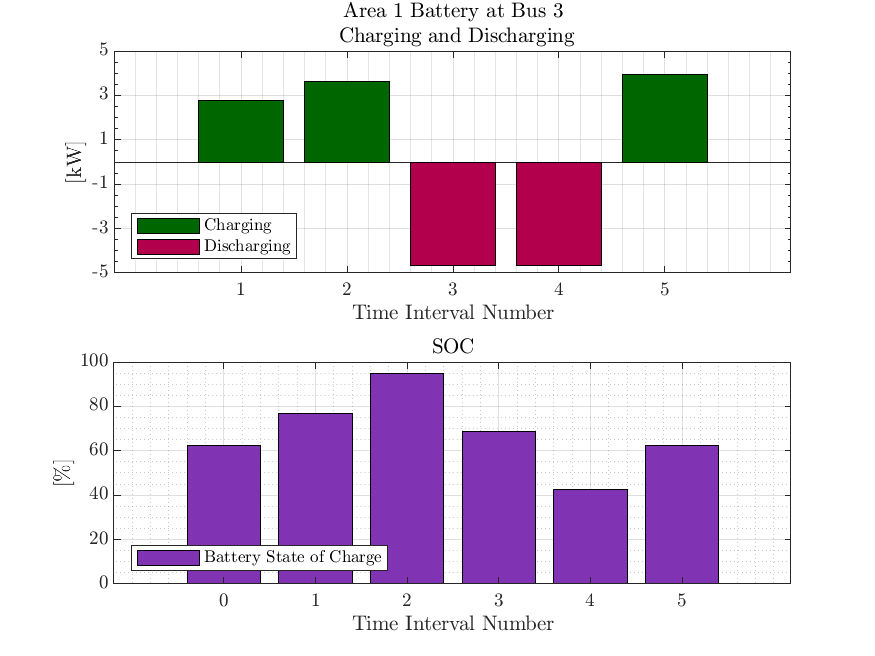
\includegraphics[width=\linewidth]{../figures/T5-pv20-batt30-genCost/dopf/BatteryPlots/macroItr_5_genCost_Battery_1_alpha_0.001.png}
%     \vspace{-5mm}
%     \caption{Charging-discharging and SOC graphs for battery at bus 3 located in Area 1 obtained by MPDOPF}
%     \label{fig:batt-plot-dopf-5-20-30-genCost}
%     \vspace{-3mm}
% \end{figure}

% \subsubsection{Workflow Analysis}
% The workflow of the MPDOPF algorithm, which involves the exchange of boundary variables between parent-child area pairs, can be seen in the convergence plots in \Cref{fig:voltage_1_2,fig:convergenceCurves-5-20-30}, with each line graph representing a particular time period in both plots. Similarly, the convergence of the objective function to its optimal value with every iteration is shown by \Cref{fig:outputConvergence-5-pv20-batt30-genCost}. From these plots, it may be noted that though initially the decision variables may be away from their optimal values, with rolling iterations they make their way to optimum values, in this case converging after 5 macro iterations. 
% The workflow of the MPDOPF algorithm, which involves the exchange of boundary variables between parent-child area pairs, is illustrated in the convergence plots in \Cref{fig:voltage_1_2,fig:convergenceCurves-5-20-30}. Each line graph represents a specific time period for both plots. Similarly, \Cref{fig:outputConvergence-5-pv20-batt30-genCost} shows the convergence of the objective function towards its optimal value over successive iterations. From these plots, we observe that although the decision variables may initially deviate from their optimal values, they gradually approach optimality with each rolling iteration, converging after 5 macro iterations in this instance.

% \begin{figure*}[h!] % convergence curves
%     \centering
%     % Row 1
%     \begin{subfigure}[b]{0.3\textwidth}
%         \centering
%         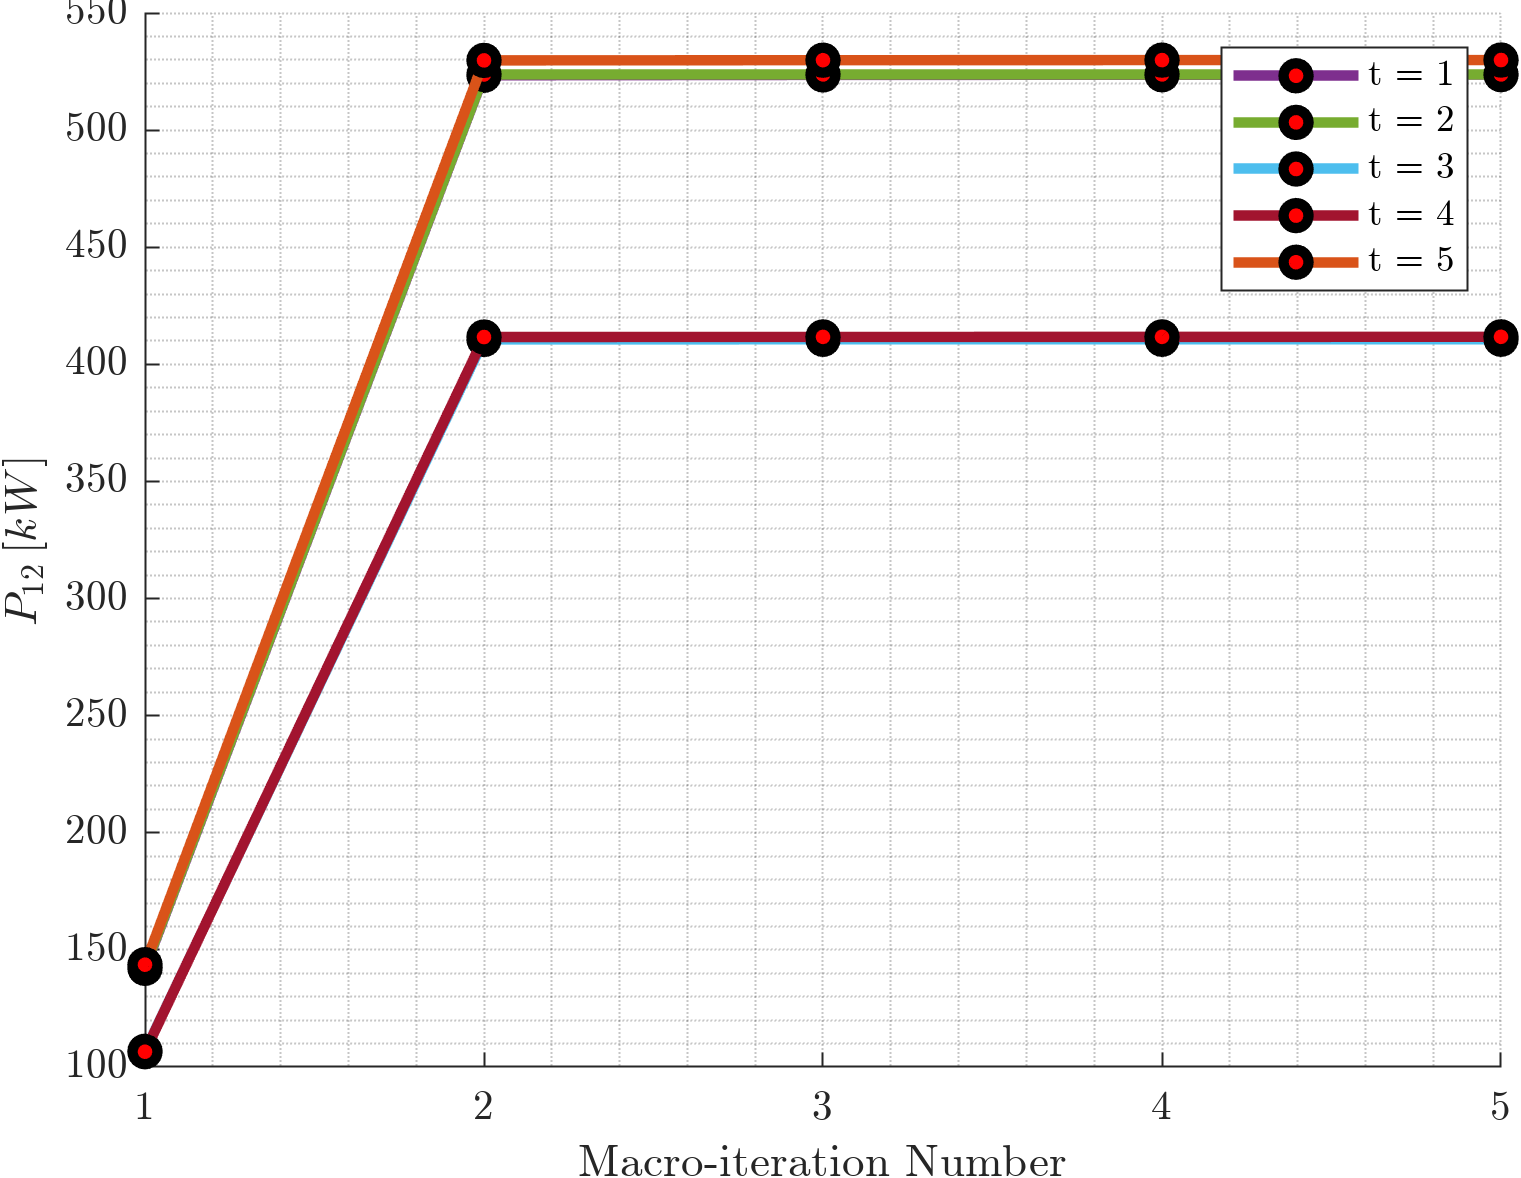
\includegraphics[width=\textwidth]{../figures/T5-pv20-batt30-genCost/dopf/convergenceCurves/BoundaryRealPower_vs_t_vs_macroItr_T_5_Areas_1_2_genCost_pv_20_batt_30_crop.png}
%         \caption{\scriptsize Real Power flowing from Area $1$ into Area $2$}
%         \label{fig:real_power_1_2}
%     \end{subfigure}
%     \hfill
%     \begin{subfigure}[b]{0.3\textwidth}
%         \centering
%         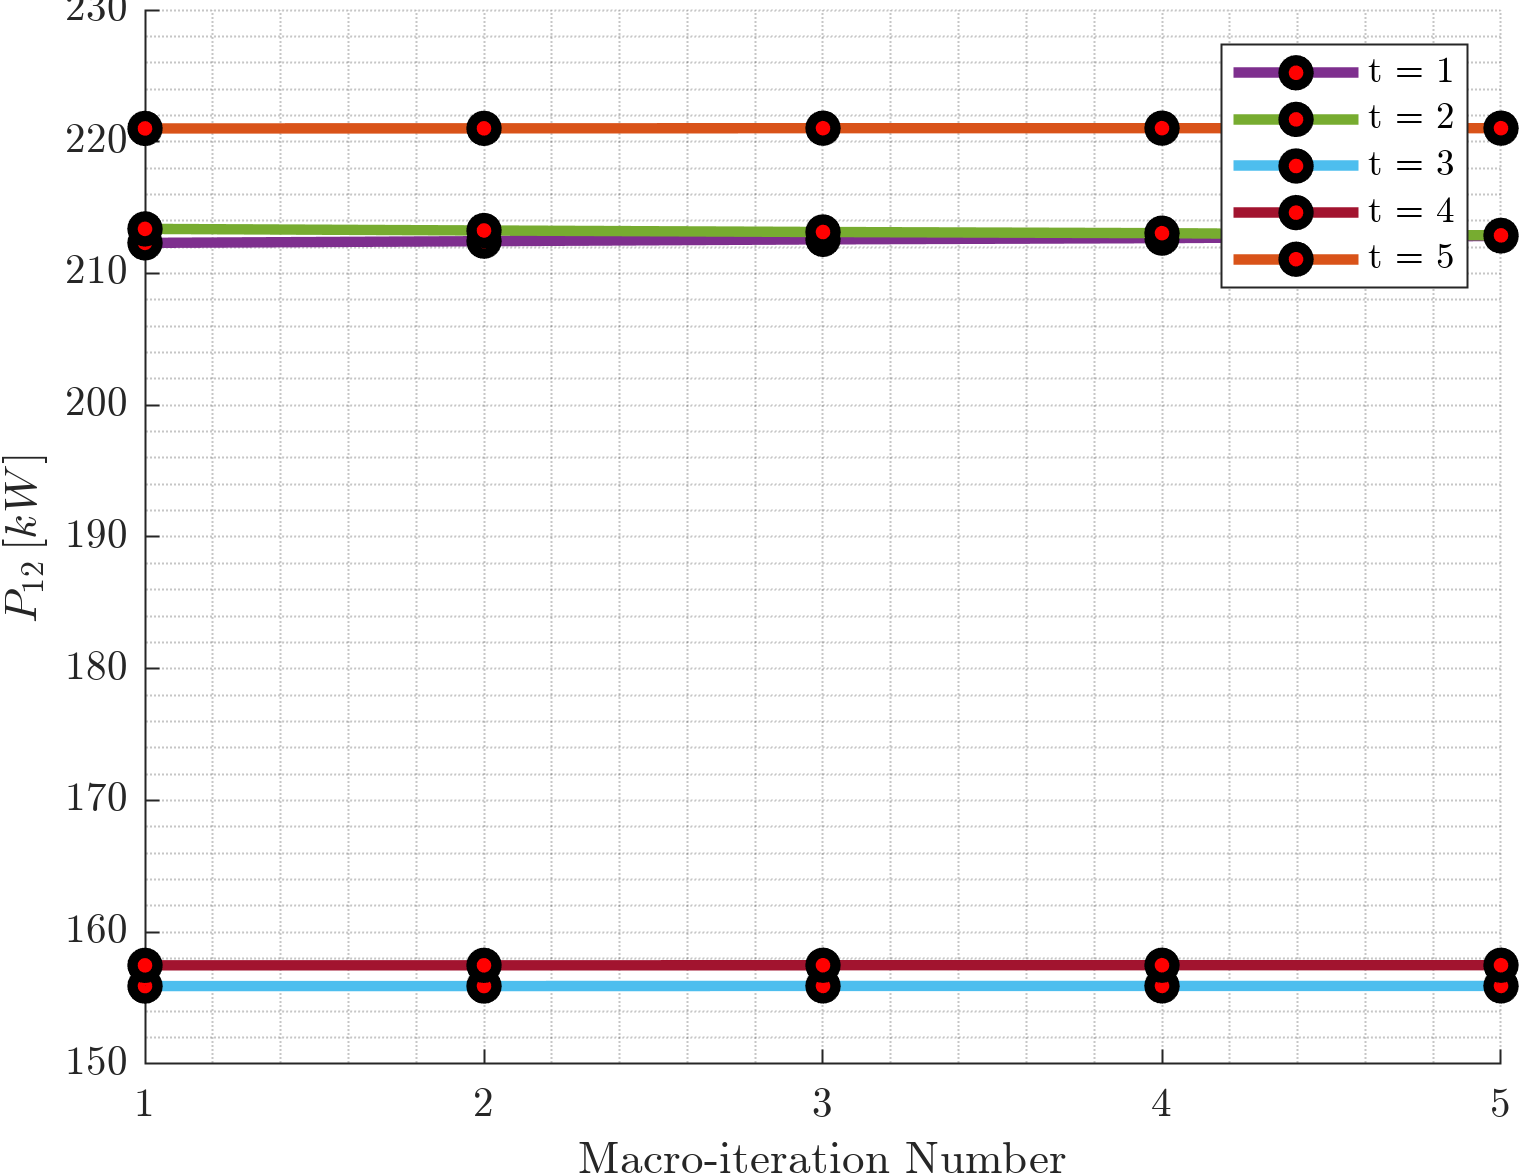
\includegraphics[width=\textwidth]{../figures/T5-pv20-batt30-genCost/dopf/convergenceCurves/BoundaryRealPower_vs_t_vs_macroItr_T_5_Areas_1_3_genCost_pv_20_batt_30_crop.png}
%         \caption{\scriptsize Real Power flowing from Area $1$ into Area $3$}
%         \label{fig:real_power_1_3}
%     \end{subfigure}
%     \hfill
%     \begin{subfigure}[b]{0.3\textwidth}
%         \centering
%         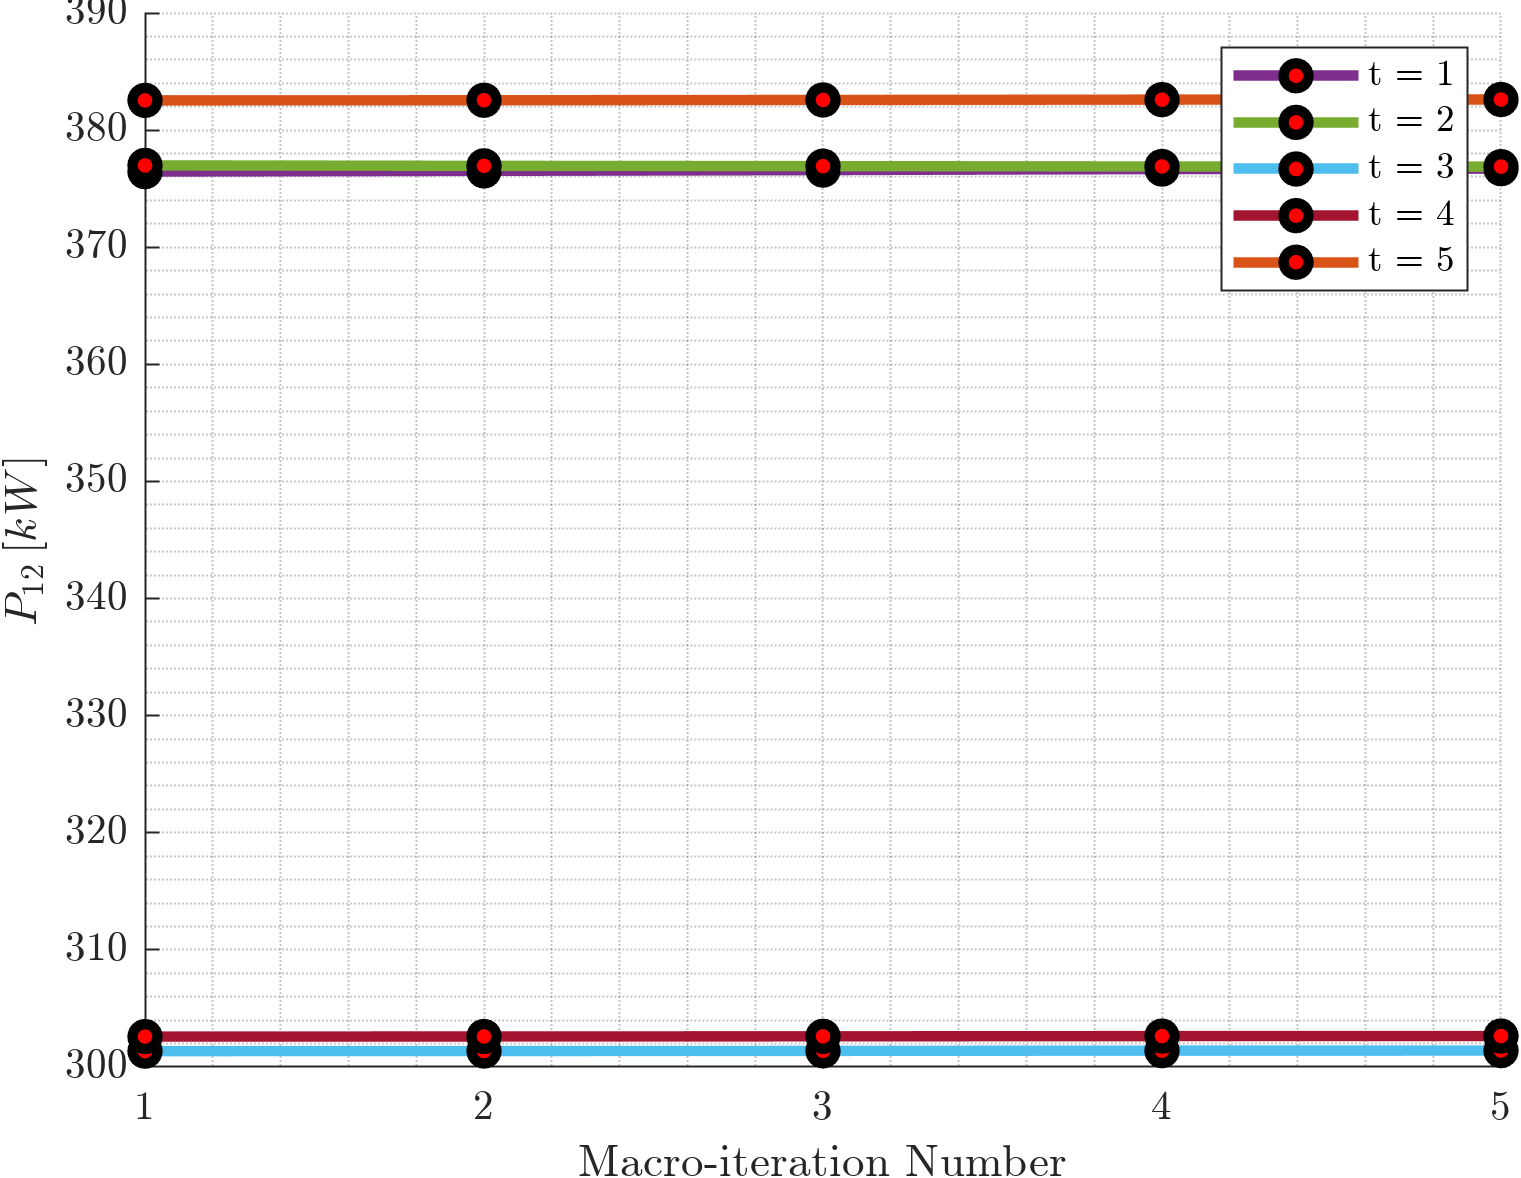
\includegraphics[width=\textwidth]{../figures/T5-pv20-batt30-genCost/dopf/convergenceCurves/BoundaryRealPower_vs_t_vs_macroItr_T_5_Areas_2_4_genCost_pv_20_batt_30_crop.png}
%         \caption{\scriptsize Real Power flowing from Area $2$ into Area $4$}
%         \label{fig:real_power_2_4}
%     \end{subfigure}
    
%     % Row 2
%     \begin{subfigure}[b]{0.3\textwidth}
%         \centering
%         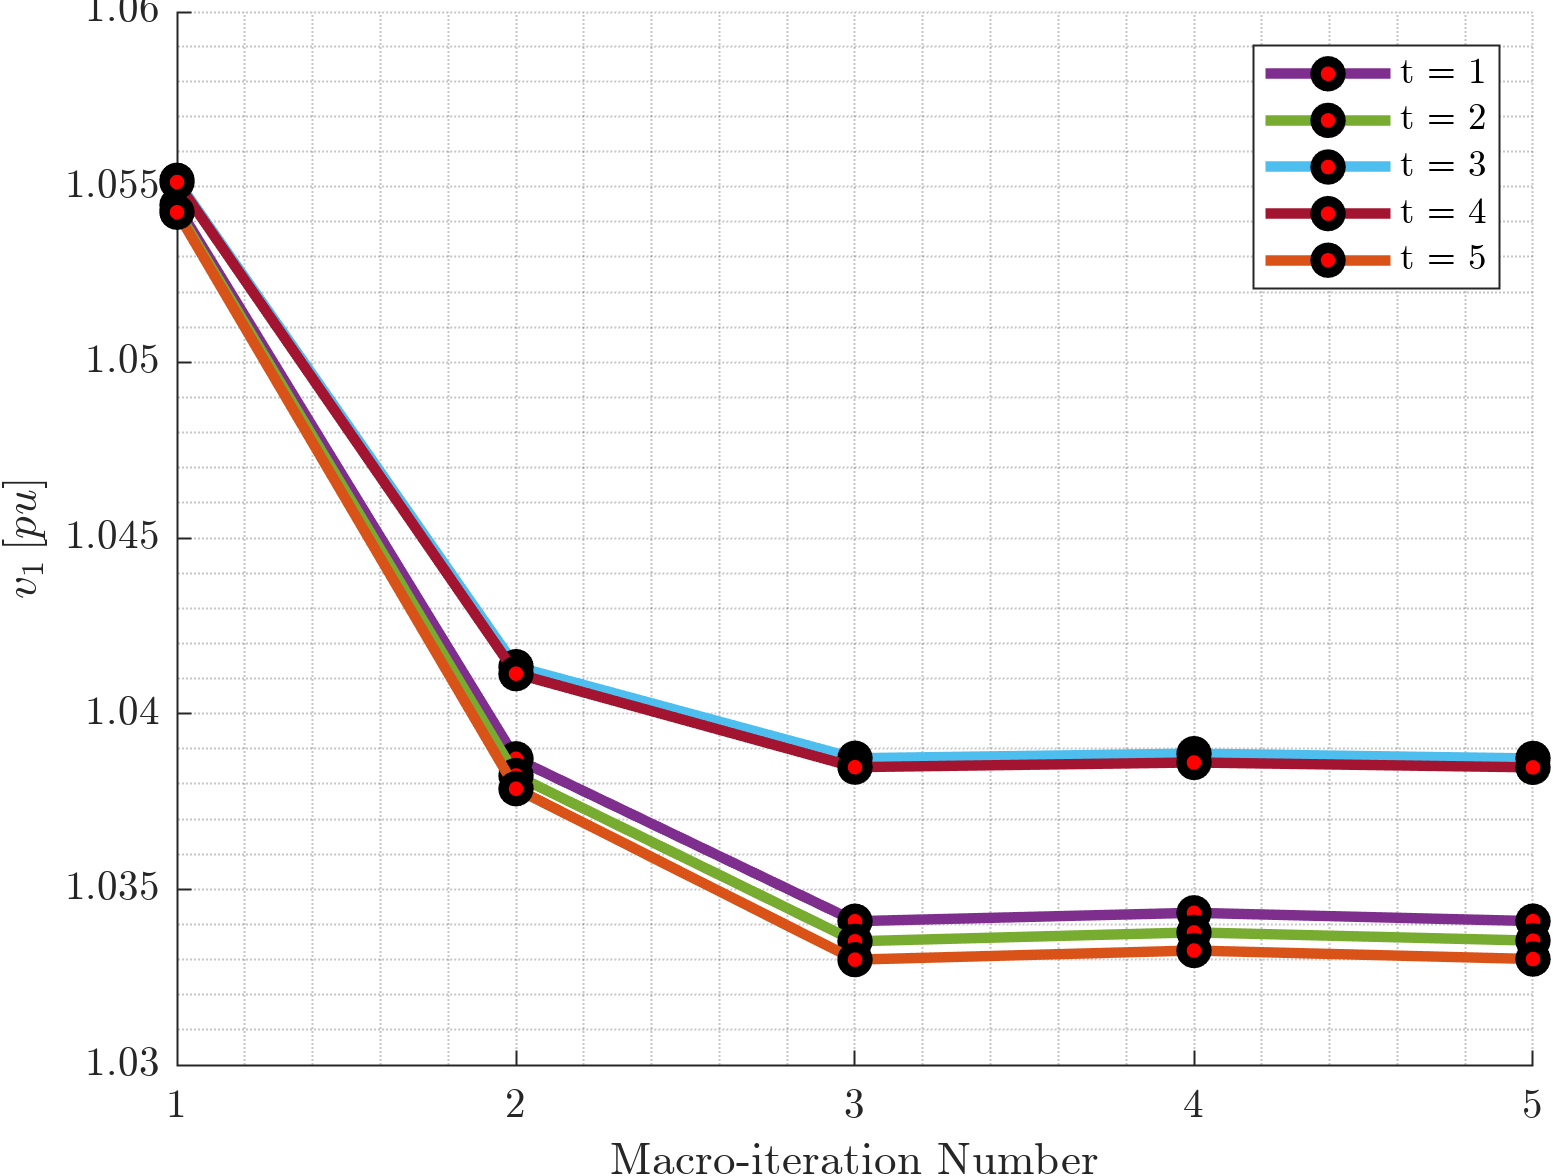
\includegraphics[width=\textwidth]{../figures/T5-pv20-batt30-genCost/dopf/convergenceCurves/BoundaryVoltage_vs_t_vs_macroItr_T_5_Areas_1_2_genCost_pv_20_batt_30_crop.png}
%         \caption{\scriptsize Voltage at the PoI of Area $1$ and Area $2$}
%         \label{fig:voltage_1_2}
%     \end{subfigure}
%     \hfill
%     \begin{subfigure}[b]{0.3\textwidth}
%         \centering
%         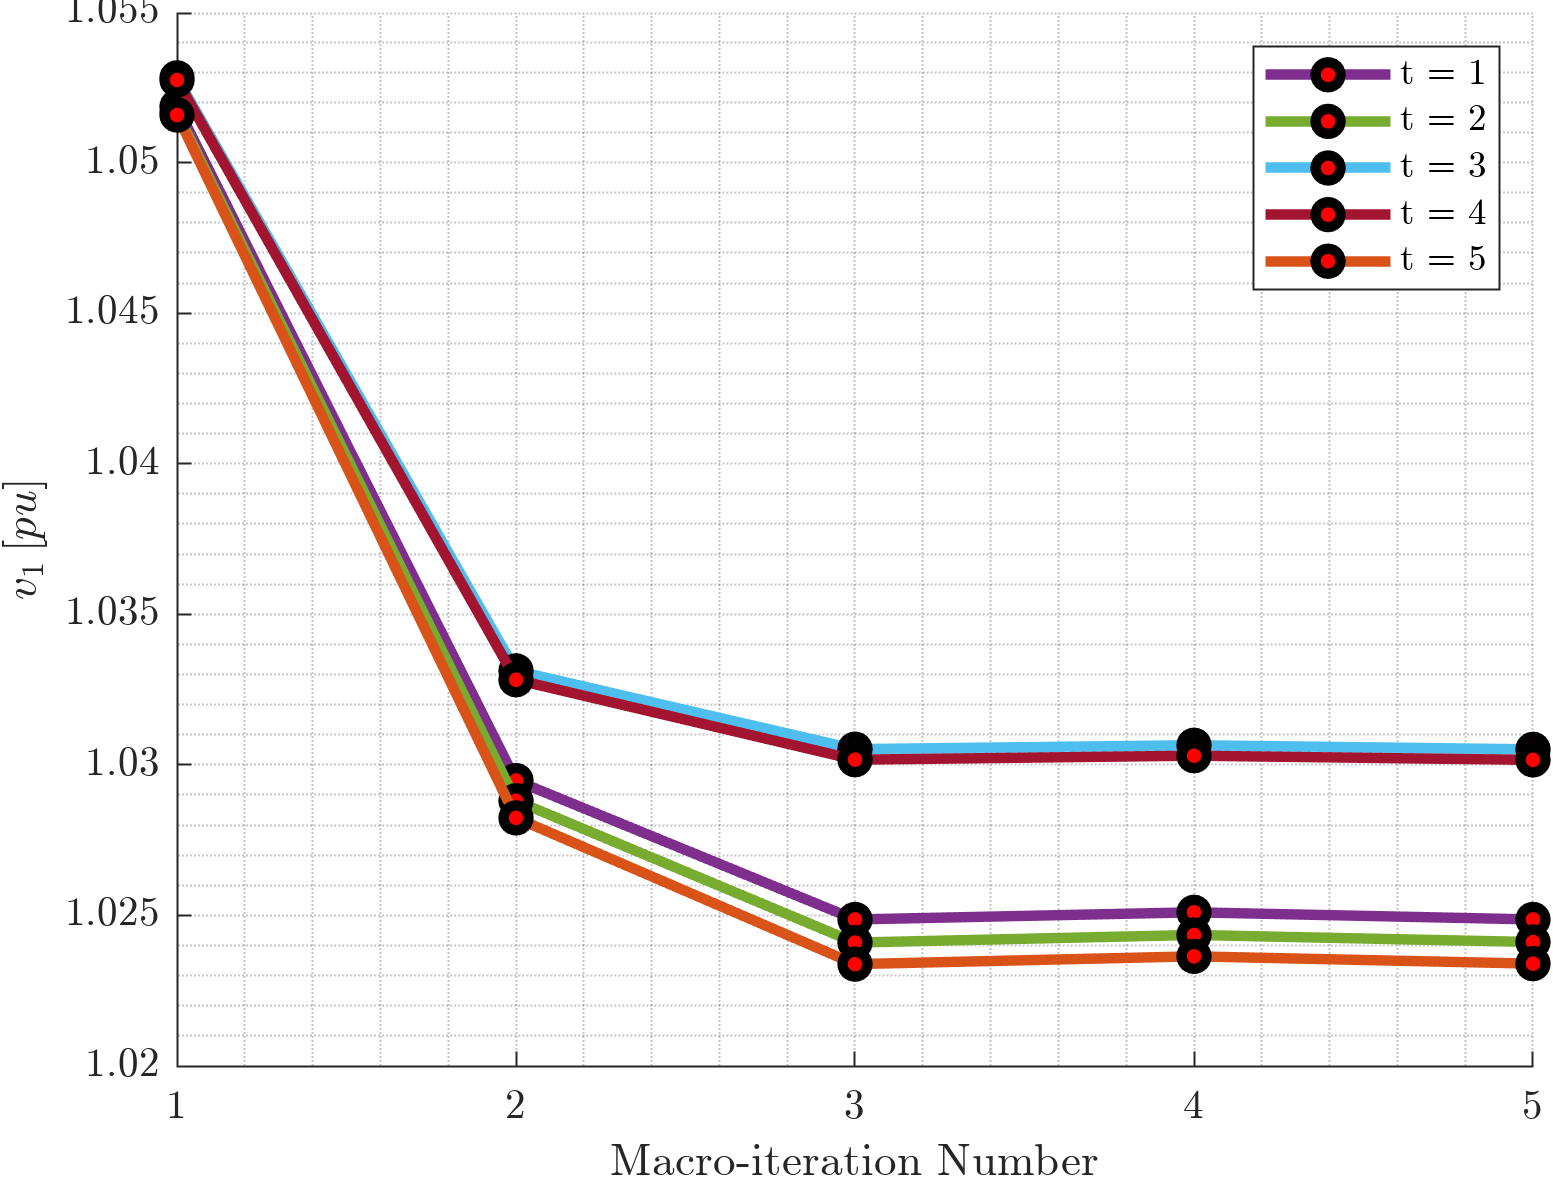
\includegraphics[width=\textwidth]{../figures/T5-pv20-batt30-genCost/dopf/convergenceCurves/BoundaryVoltage_vs_t_vs_macroItr_T_5_Areas_1_3_genCost_pv_20_batt_30_crop.png}
%         \caption{\scriptsize Voltage at the PoI of Area $1$ and Area $3$}
%         \label{fig:voltage_1_3}
%     \end{subfigure}
%     \hfill
%     \begin{subfigure}[b]{0.3\textwidth}
%         \centering
%         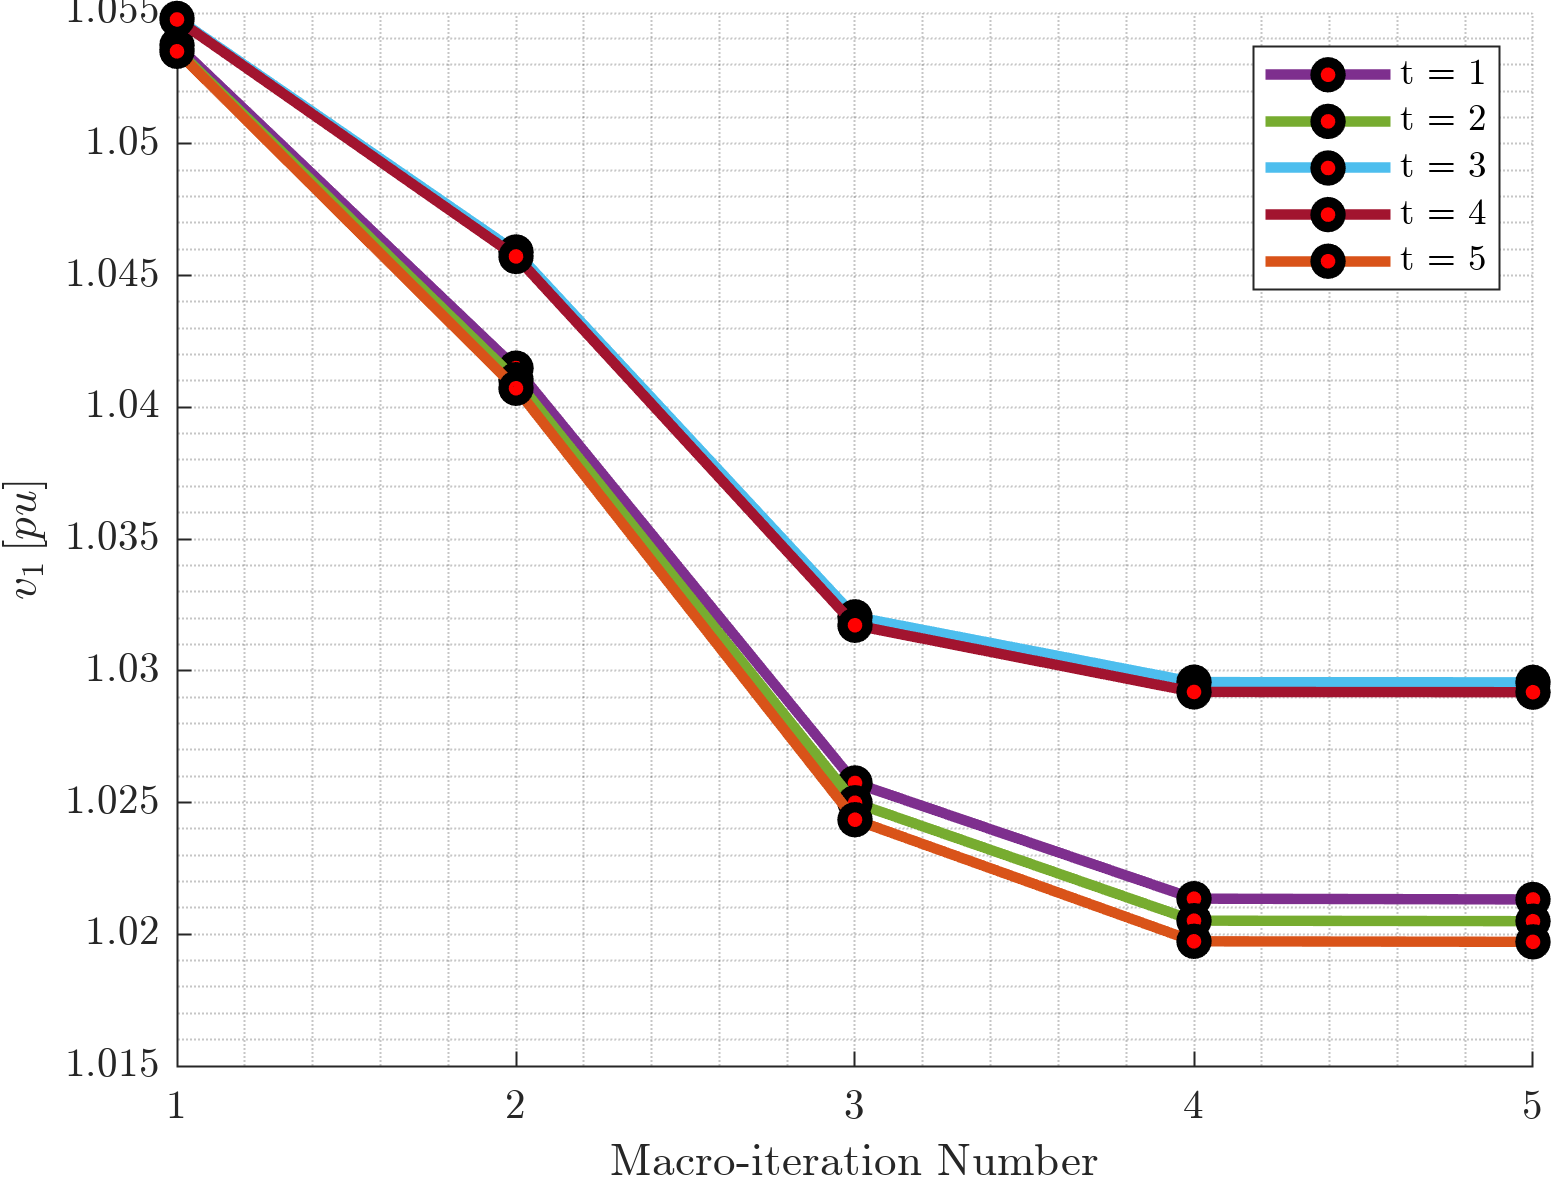
\includegraphics[width=\textwidth]{../figures/T5-pv20-batt30-genCost/dopf/convergenceCurves/BoundaryVoltage_vs_t_vs_macroItr_T_5_Areas_2_4_genCost_pv_20_batt_30_crop.png}
%         \caption{\scriptsize Voltage at the PoI of Area $2$ and Area $4$}
%         \label{fig:voltage_2_4}
%     \end{subfigure}

%     \caption{Convergence of Boundary variables with every iteration. Each plot represents a particular variable exchanged between a pair of connected areas. Each line graph within a plot represents a particular time period.}
%     \label{fig:convergenceCurves-5-20-30}
% \end{figure*}

% \begin{figure*}[h] % convergence curves
%     \centering
%     % Row 1
%     \begin{subfigure}[b]{0.3\textwidth}
%         \centering
%         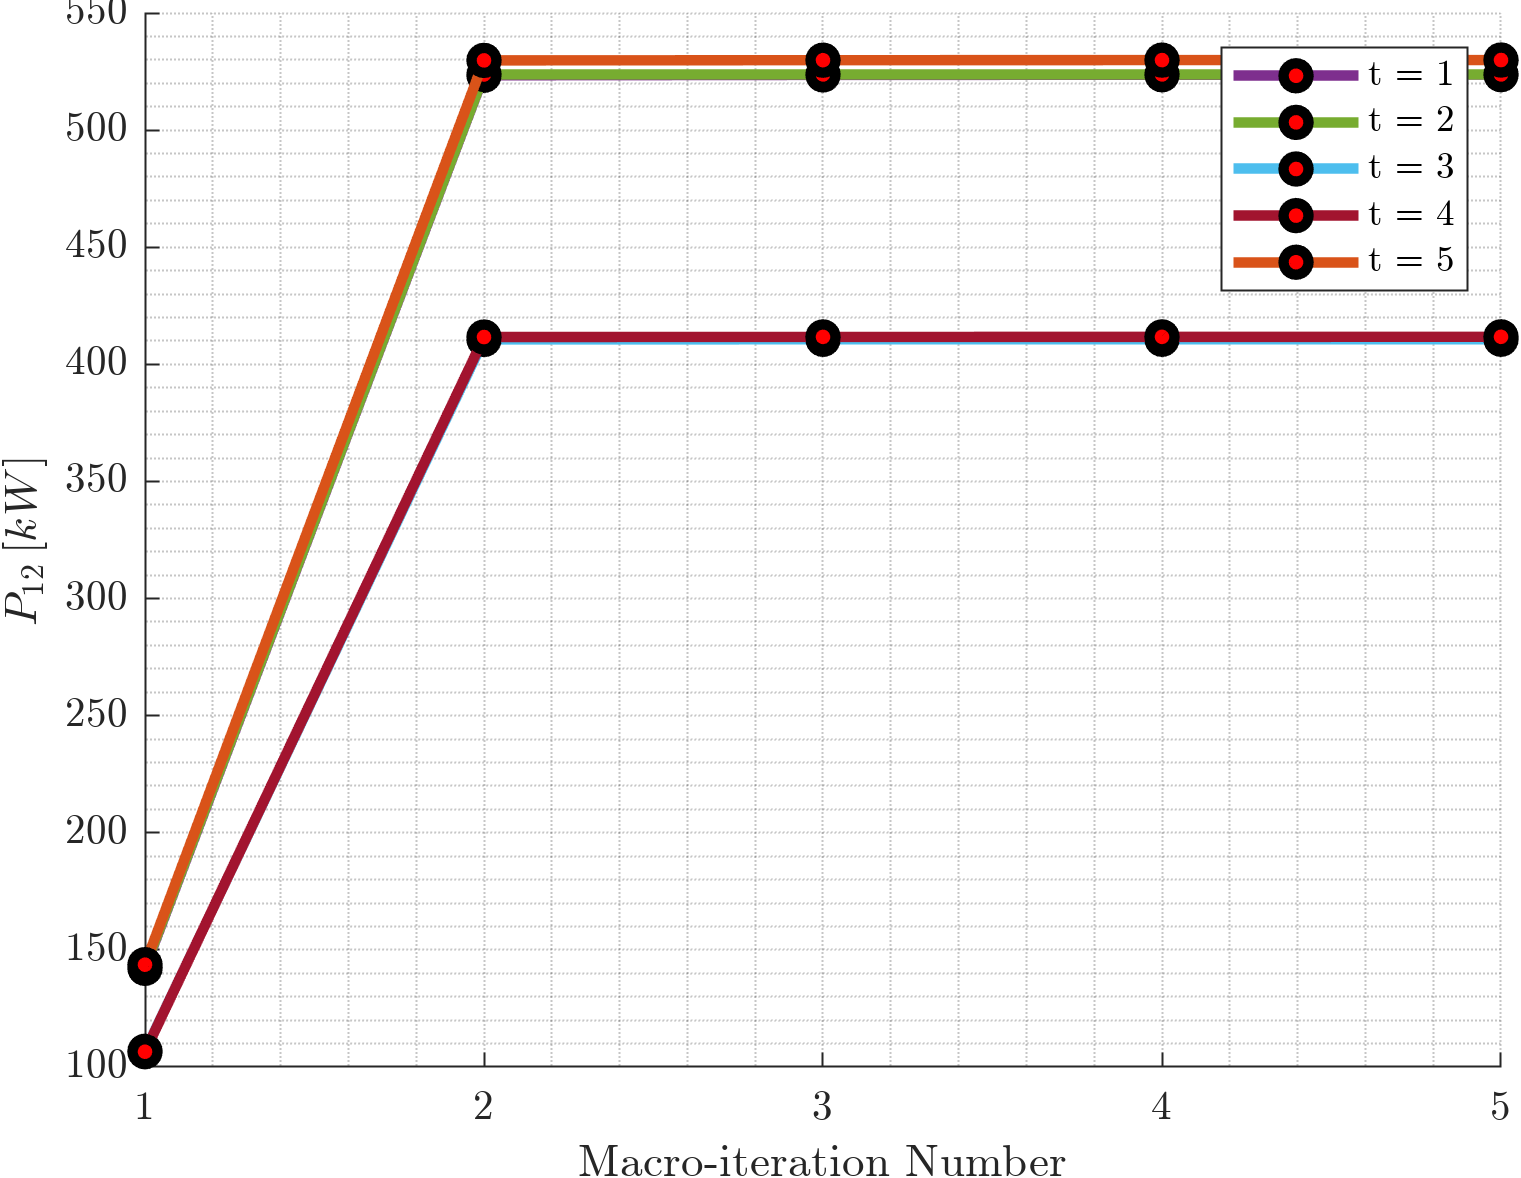
\includegraphics[scale=0.3]{../figures/T5-pv20-batt30-genCost/dopf/convergenceCurves/BoundaryRealPower_vs_t_vs_macroItr_T_5_Areas_1_2_genCost_pv_20_batt_30_crop.png}
%         \caption{\scriptsize Real Power flowing from Area $1$ into Area $2$}
%         \label{fig:real_power_1_2}
%     \end{subfigure}
%     \hfill
%     \begin{subfigure}[b]{0.3\textwidth}
%         \centering
%         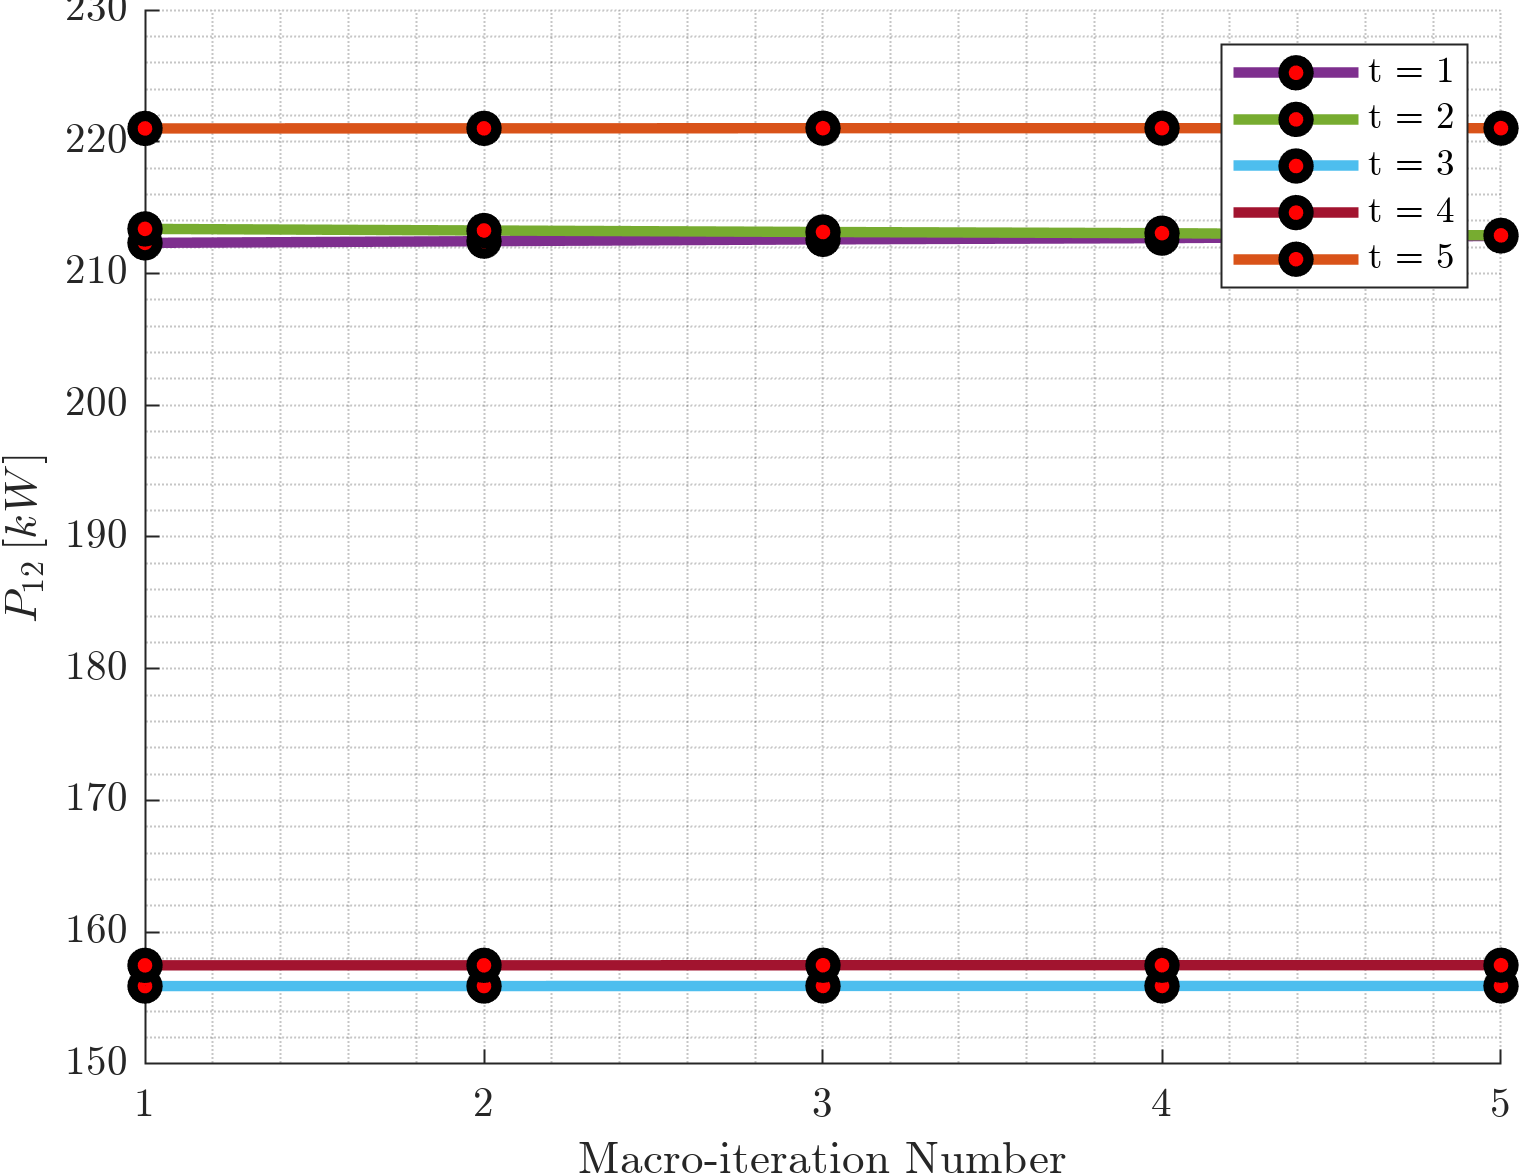
\includegraphics[scale=0.3]{../figures/T5-pv20-batt30-genCost/dopf/convergenceCurves/BoundaryRealPower_vs_t_vs_macroItr_T_5_Areas_1_3_genCost_pv_20_batt_30_crop.png}
%         \caption{\scriptsize Real Power flowing from Area $1$ into Area $3$}
%         \label{fig:real_power_1_3}
%     \end{subfigure}
%     \hfill
%     \begin{subfigure}[b]{0.3\textwidth}
%         \centering
%         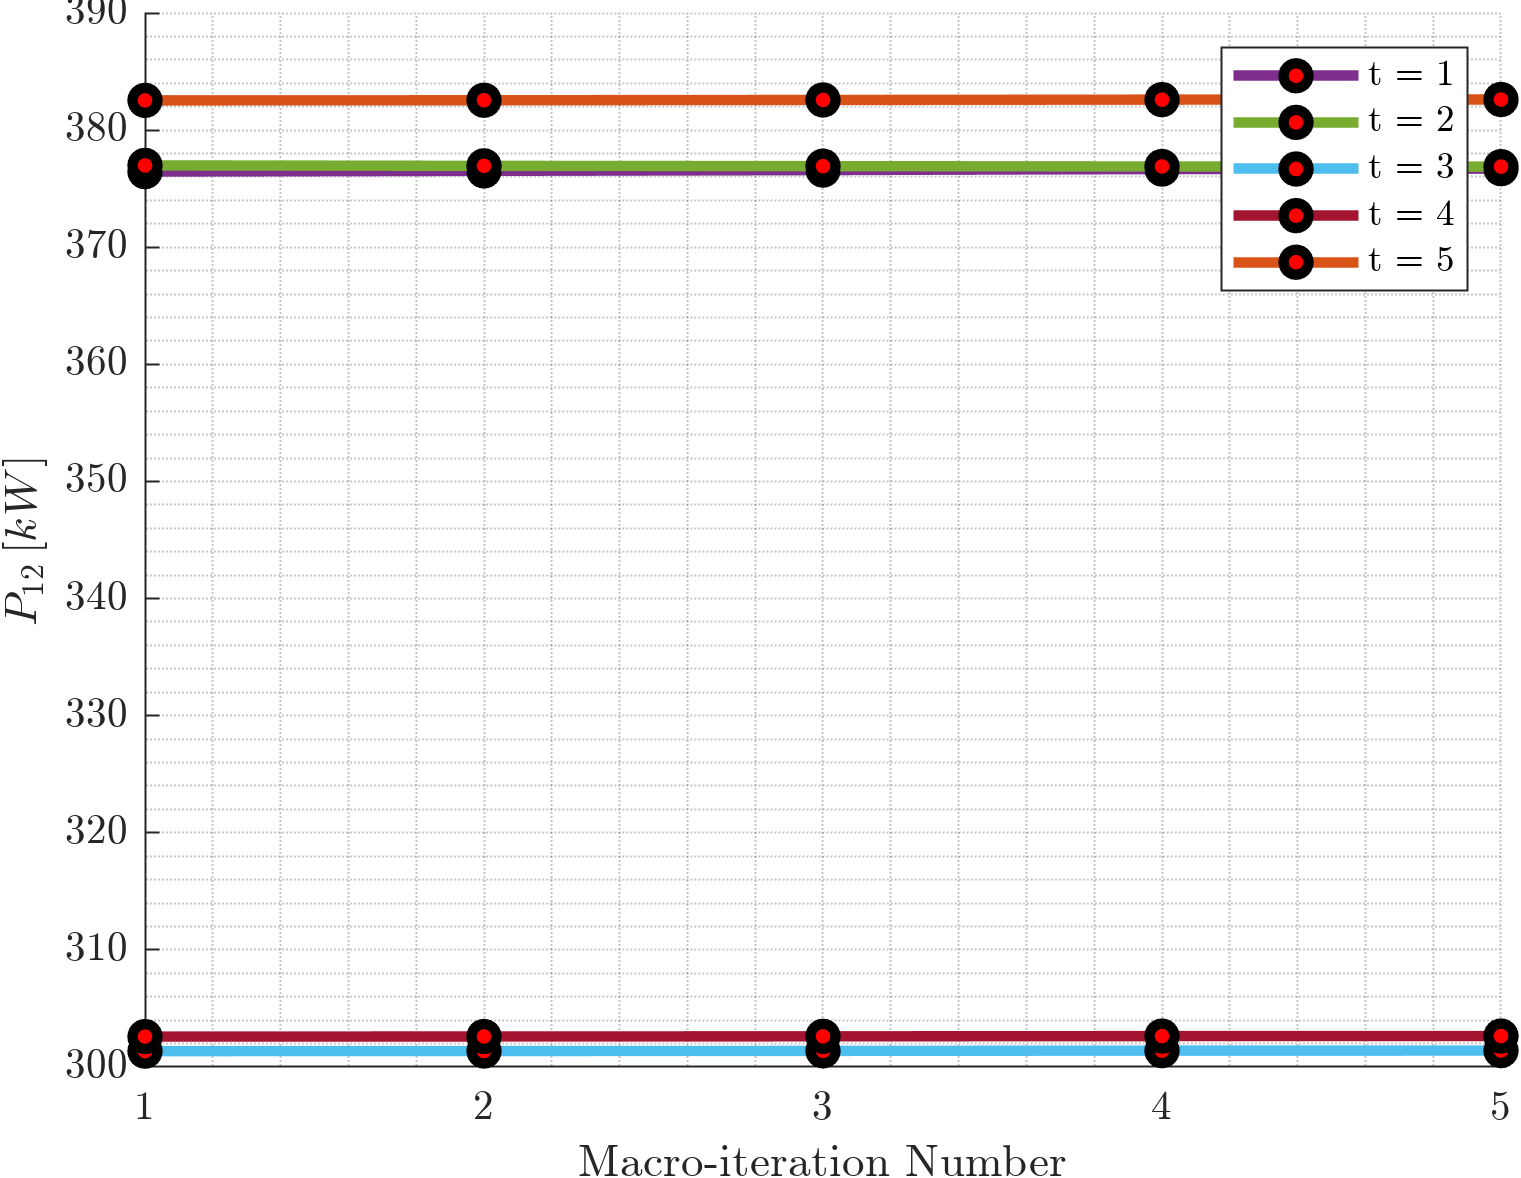
\includegraphics[scale=0.3]{../figures/T5-pv20-batt30-genCost/dopf/convergenceCurves/BoundaryRealPower_vs_t_vs_macroItr_T_5_Areas_2_4_genCost_pv_20_batt_30_crop.png}
%         \caption{\scriptsize Real Power flowing from Area $2$ into Area $4$}
%         \label{fig:real_power_2_4}
%     \end{subfigure}
    
%     % Row 2
%     \begin{subfigure}[b]{0.3\textwidth}
%         \centering
%         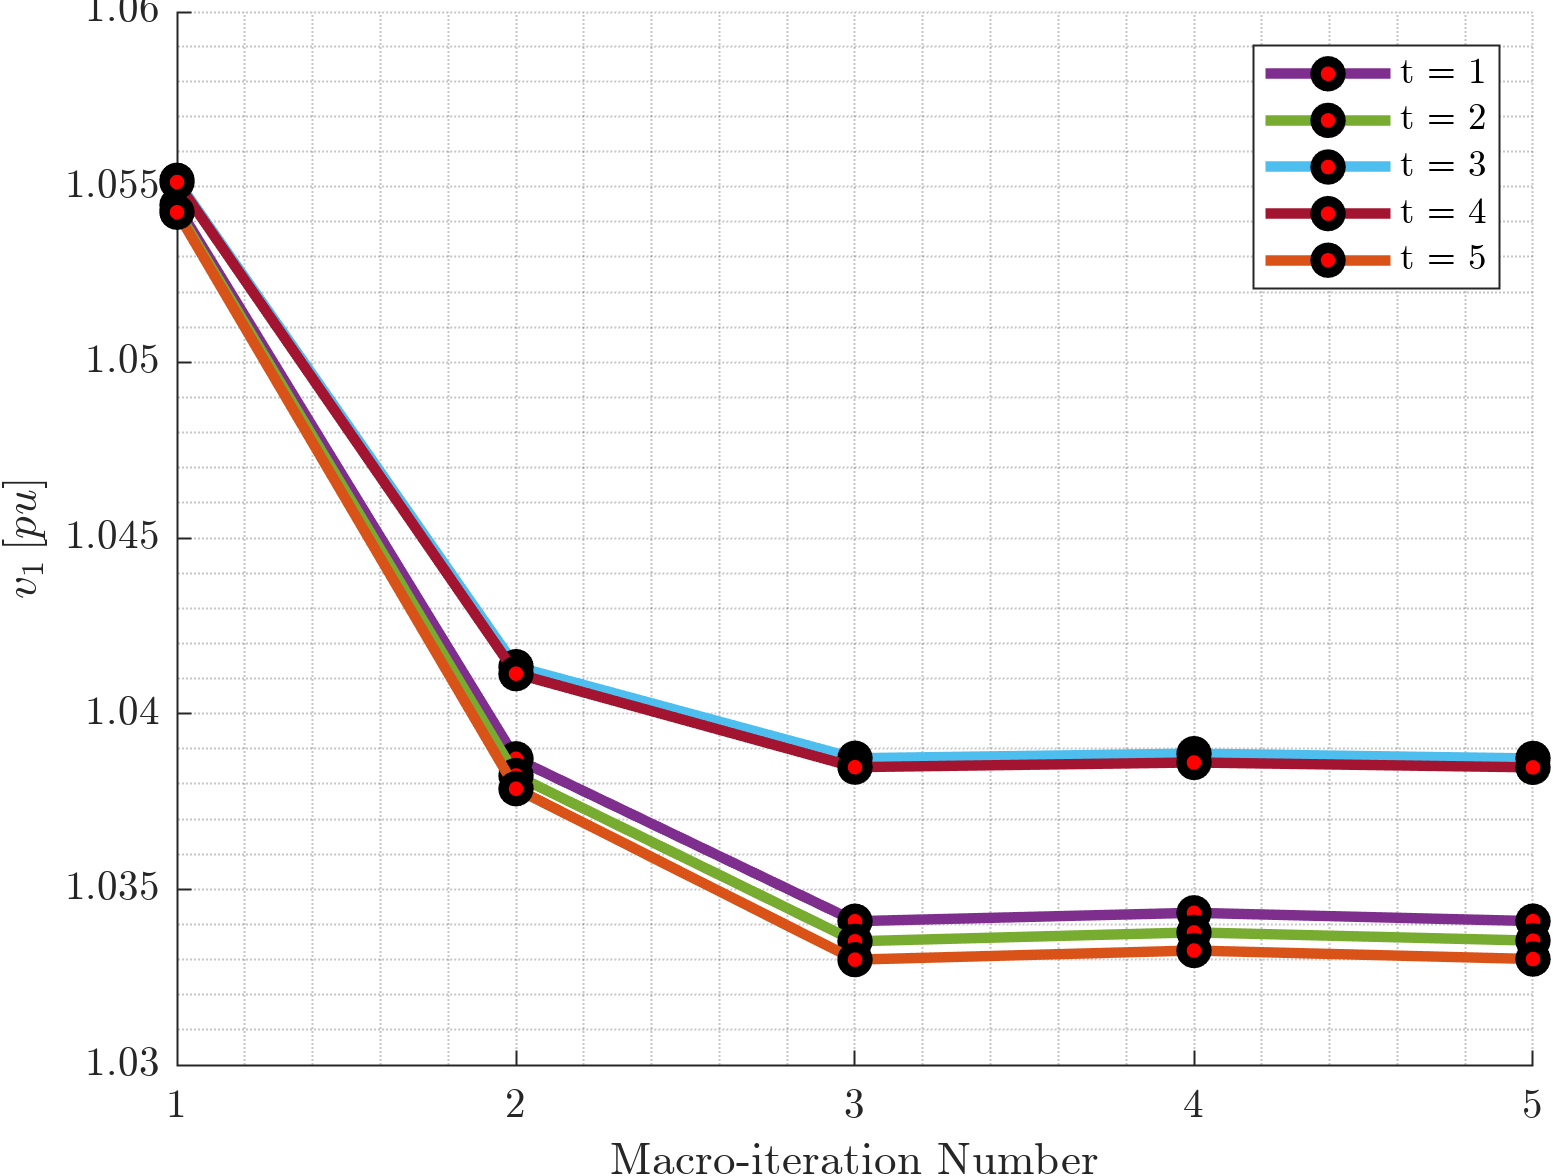
\includegraphics[scale=0.3]{../figures/T5-pv20-batt30-genCost/dopf/convergenceCurves/BoundaryVoltage_vs_t_vs_macroItr_T_5_Areas_1_2_genCost_pv_20_batt_30_crop.png}
%         \caption{\scriptsize Voltage at the PoI of Area $1$ and Area $2$}
%         \label{fig:voltage_1_2}
%     \end{subfigure}
%     \hfill
%     \begin{subfigure}[b]{0.3\textwidth}
%         \centering
%         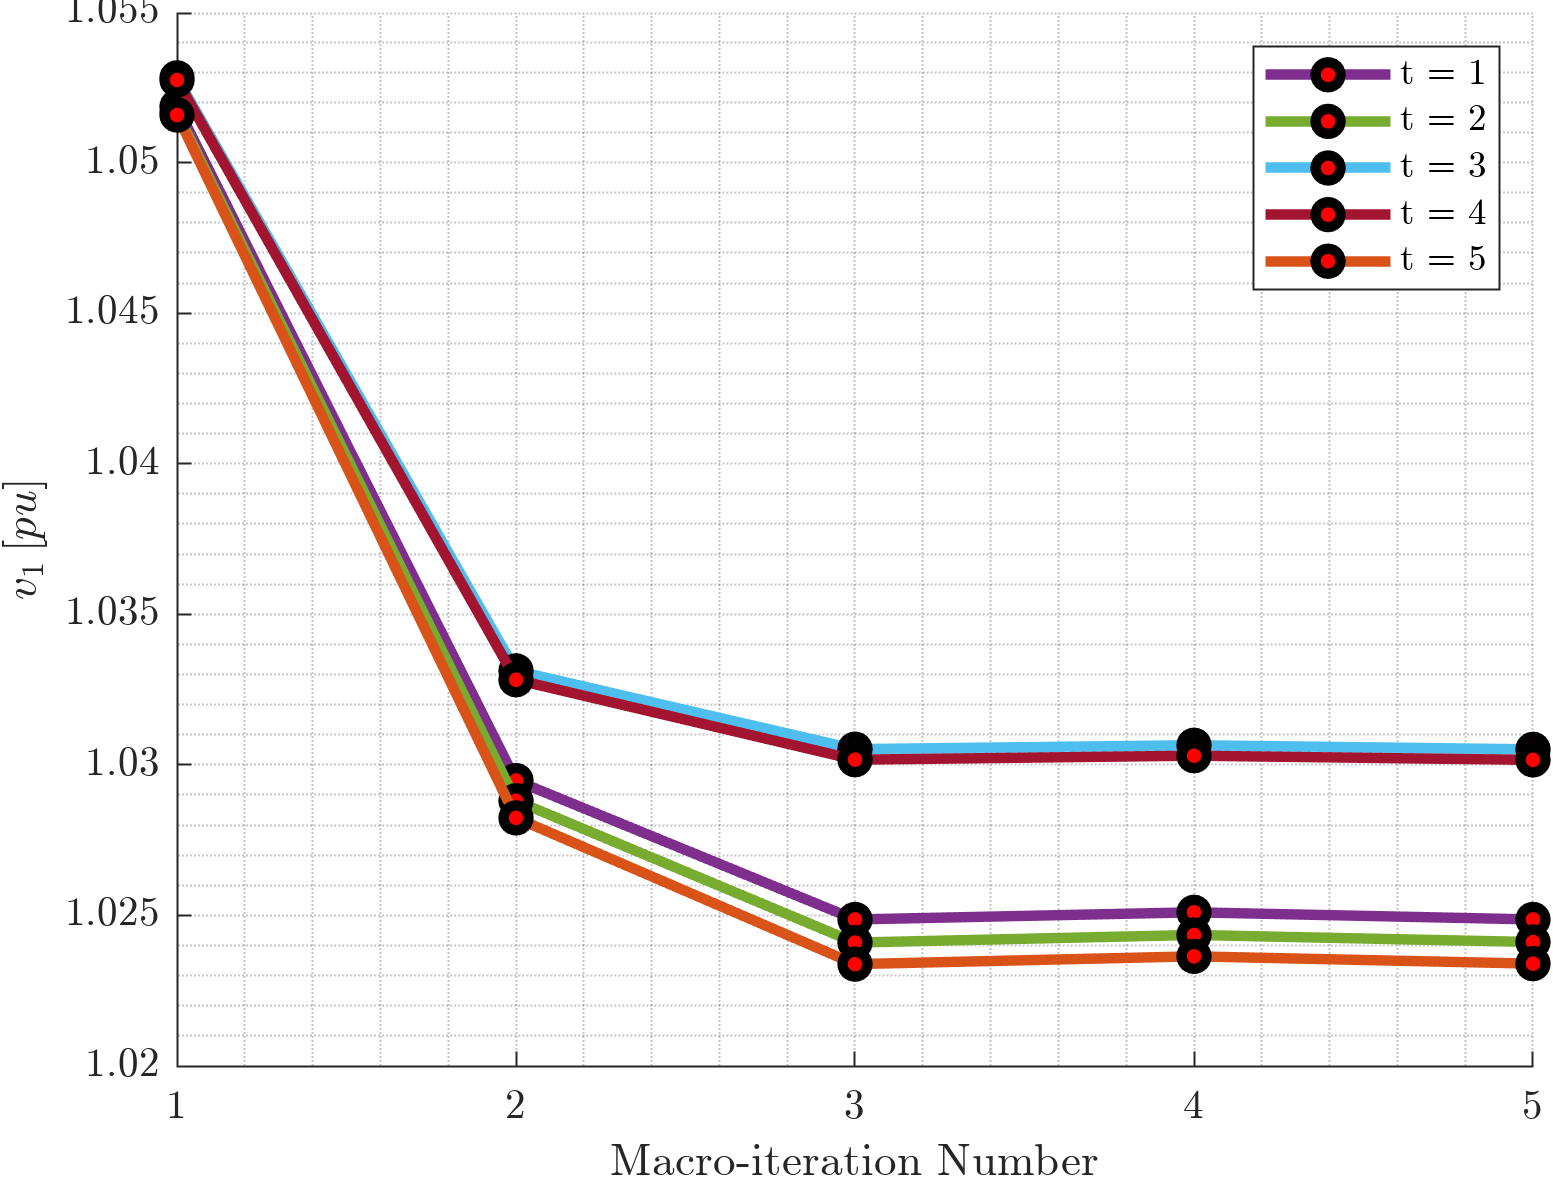
\includegraphics[scale=0.3]{../figures/T5-pv20-batt30-genCost/dopf/convergenceCurves/BoundaryVoltage_vs_t_vs_macroItr_T_5_Areas_1_3_genCost_pv_20_batt_30_crop.png}
%         \caption{\scriptsize Voltage at the PoI of Area $1$ and Area $3$}
%         \label{fig:voltage_1_3}
%     \end{subfigure}
%     \hfill
%     \begin{subfigure}[b]{0.3\textwidth}
%         \centering
%         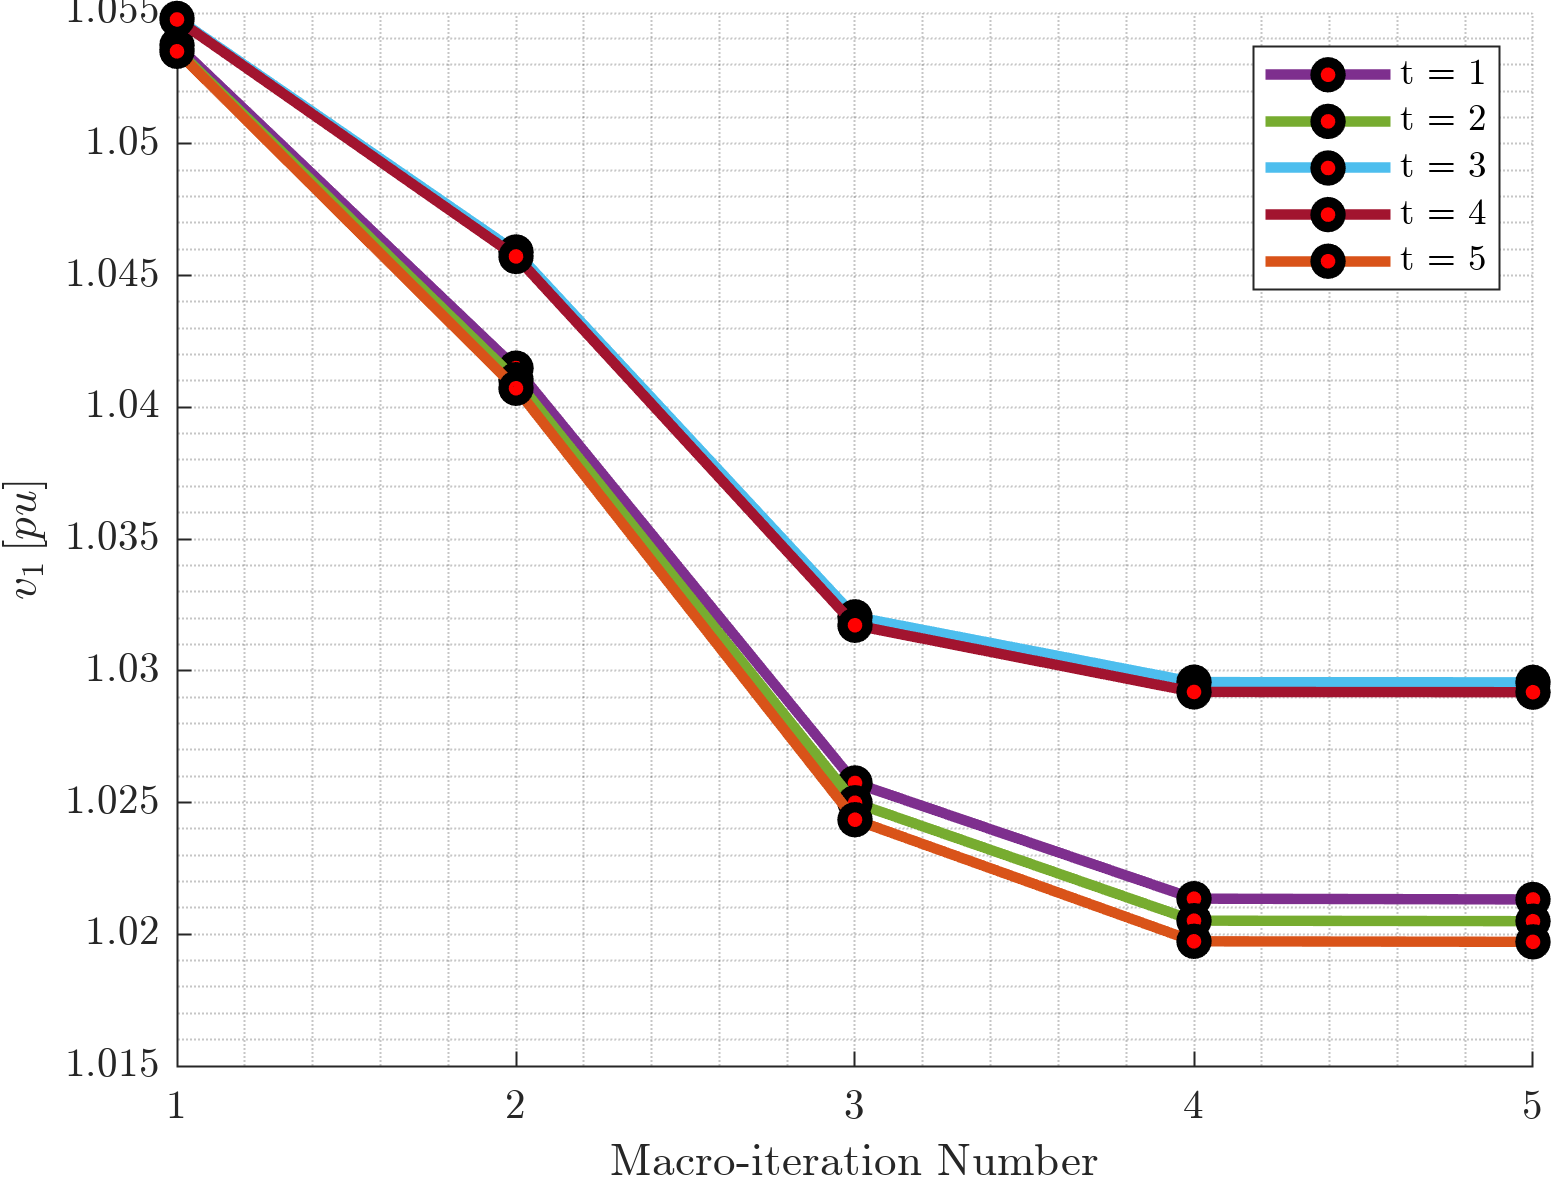
\includegraphics[scale=0.3]{../figures/T5-pv20-batt30-genCost/dopf/convergenceCurves/BoundaryVoltage_vs_t_vs_macroItr_T_5_Areas_2_4_genCost_pv_20_batt_30_crop.png}
%         \caption{\scriptsize Voltage at the PoI of Area $2$ and Area $4$}
%         \label{fig:voltage_2_4}
%     \end{subfigure}

%     \caption{Convergence of Boundary variables with every iteration. Each plot represents a particular variable exchanged between a pair of connected areas. Each line graph within a plot represents a particular time period.}
%     \label{fig:convergenceCurves-5-20-30}
% \end{figure*}

% \begin{figure}[H] % convergence curves
%     \centering
%     % Row 1
%     \begin{subfigure}[b]{0.3\textwidth}
%         \centering
%         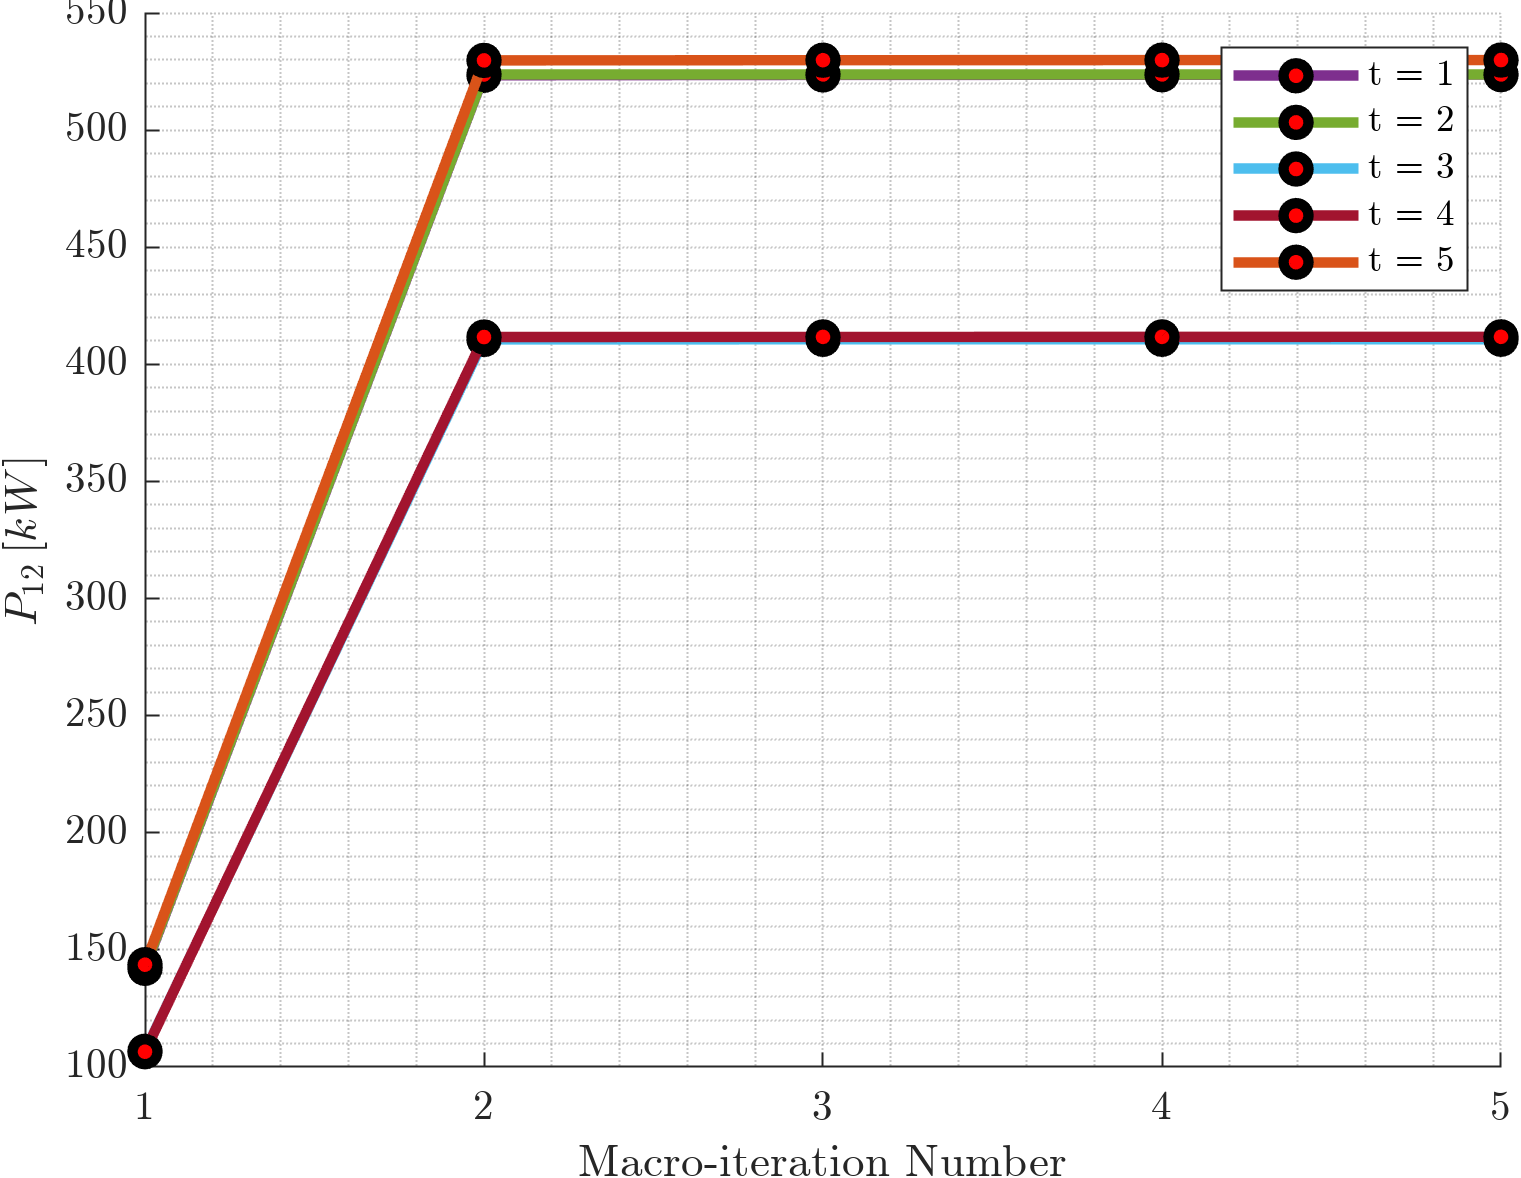
\includegraphics[width=\textwidth,height=0.6\textwidth]{../figures/T5-pv20-batt30-genCost/dopf/convergenceCurves/BoundaryRealPower_vs_t_vs_macroItr_T_5_Areas_1_2_genCost_pv_20_batt_30_crop.png}
%         \caption{\scriptsize Real Power flowing from Area $1$ into Area $2$}
%         \label{fig:real_power_1_2}
%     \end{subfigure}
%     \hfill
%     \begin{subfigure}[b]{0.3\textwidth}
%         \centering
%         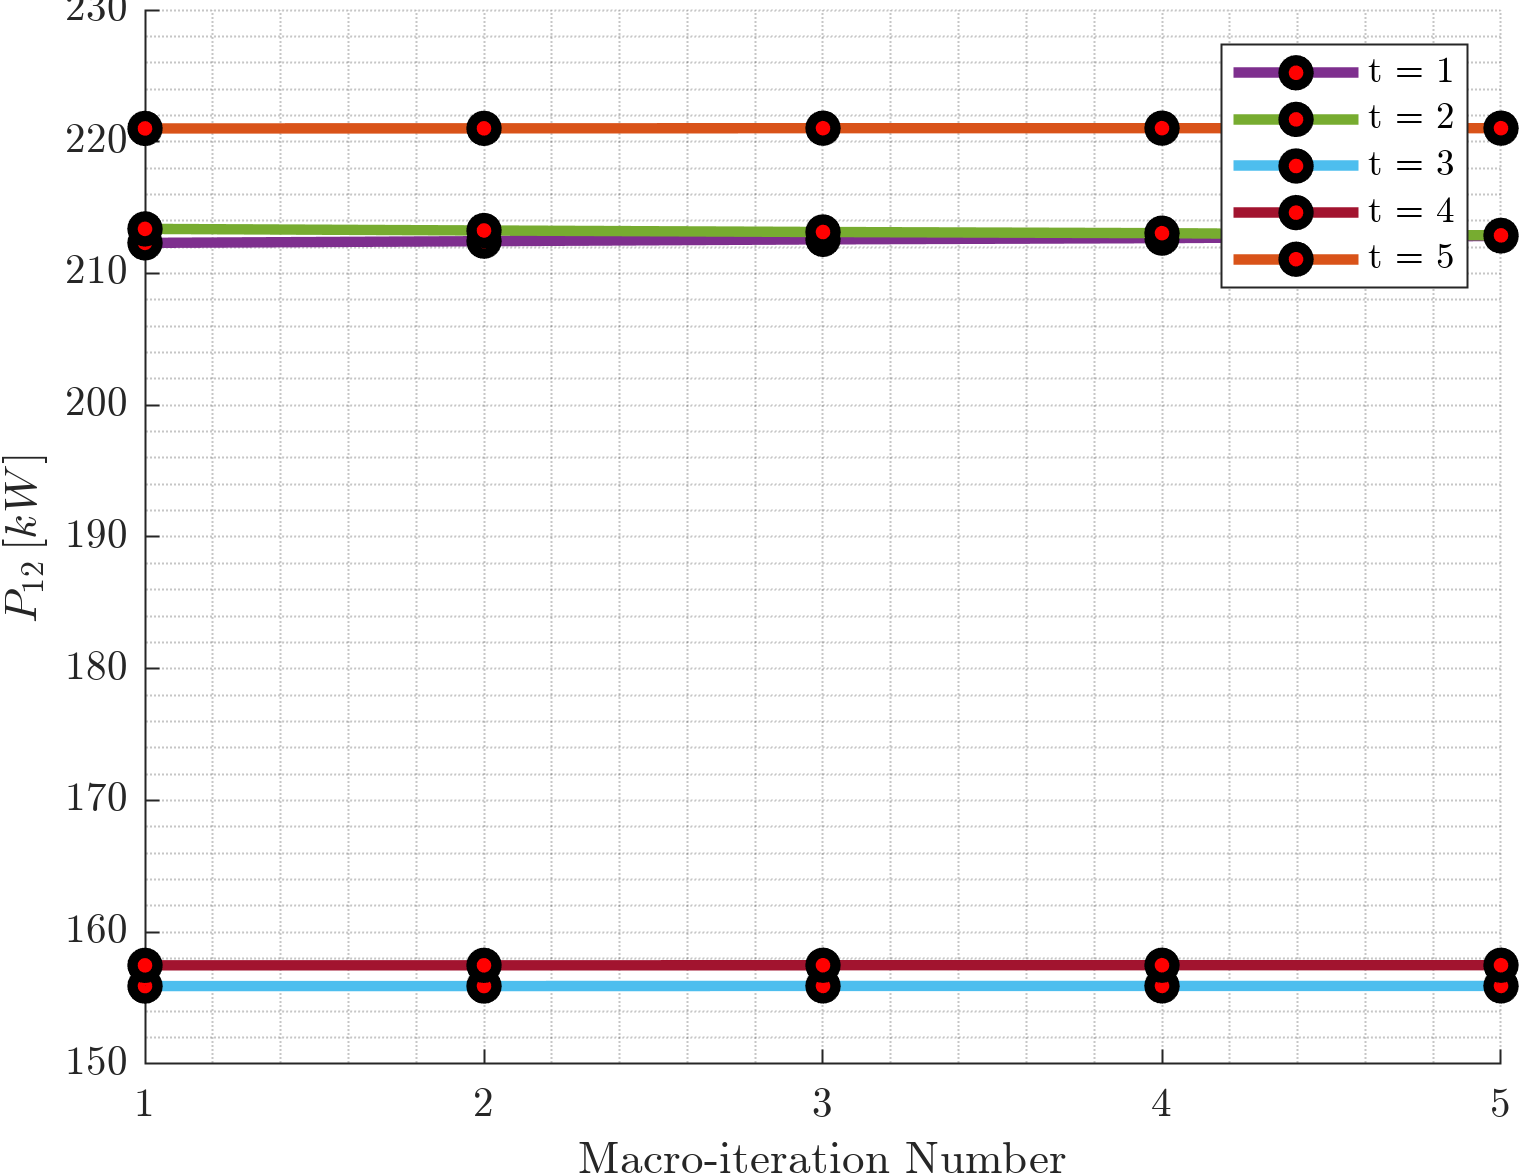
\includegraphics[width=\textwidth,height=0.6\textwidth]{../figures/T5-pv20-batt30-genCost/dopf/convergenceCurves/BoundaryRealPower_vs_t_vs_macroItr_T_5_Areas_1_3_genCost_pv_20_batt_30_crop.png}
%         \caption{\scriptsize Real Power flowing from Area $1$ into Area $3$}
%         \label{fig:real_power_1_3}
%     \end{subfigure}
%     \hfill
%     \begin{subfigure}[b]{0.3\textwidth}
%         \centering
%         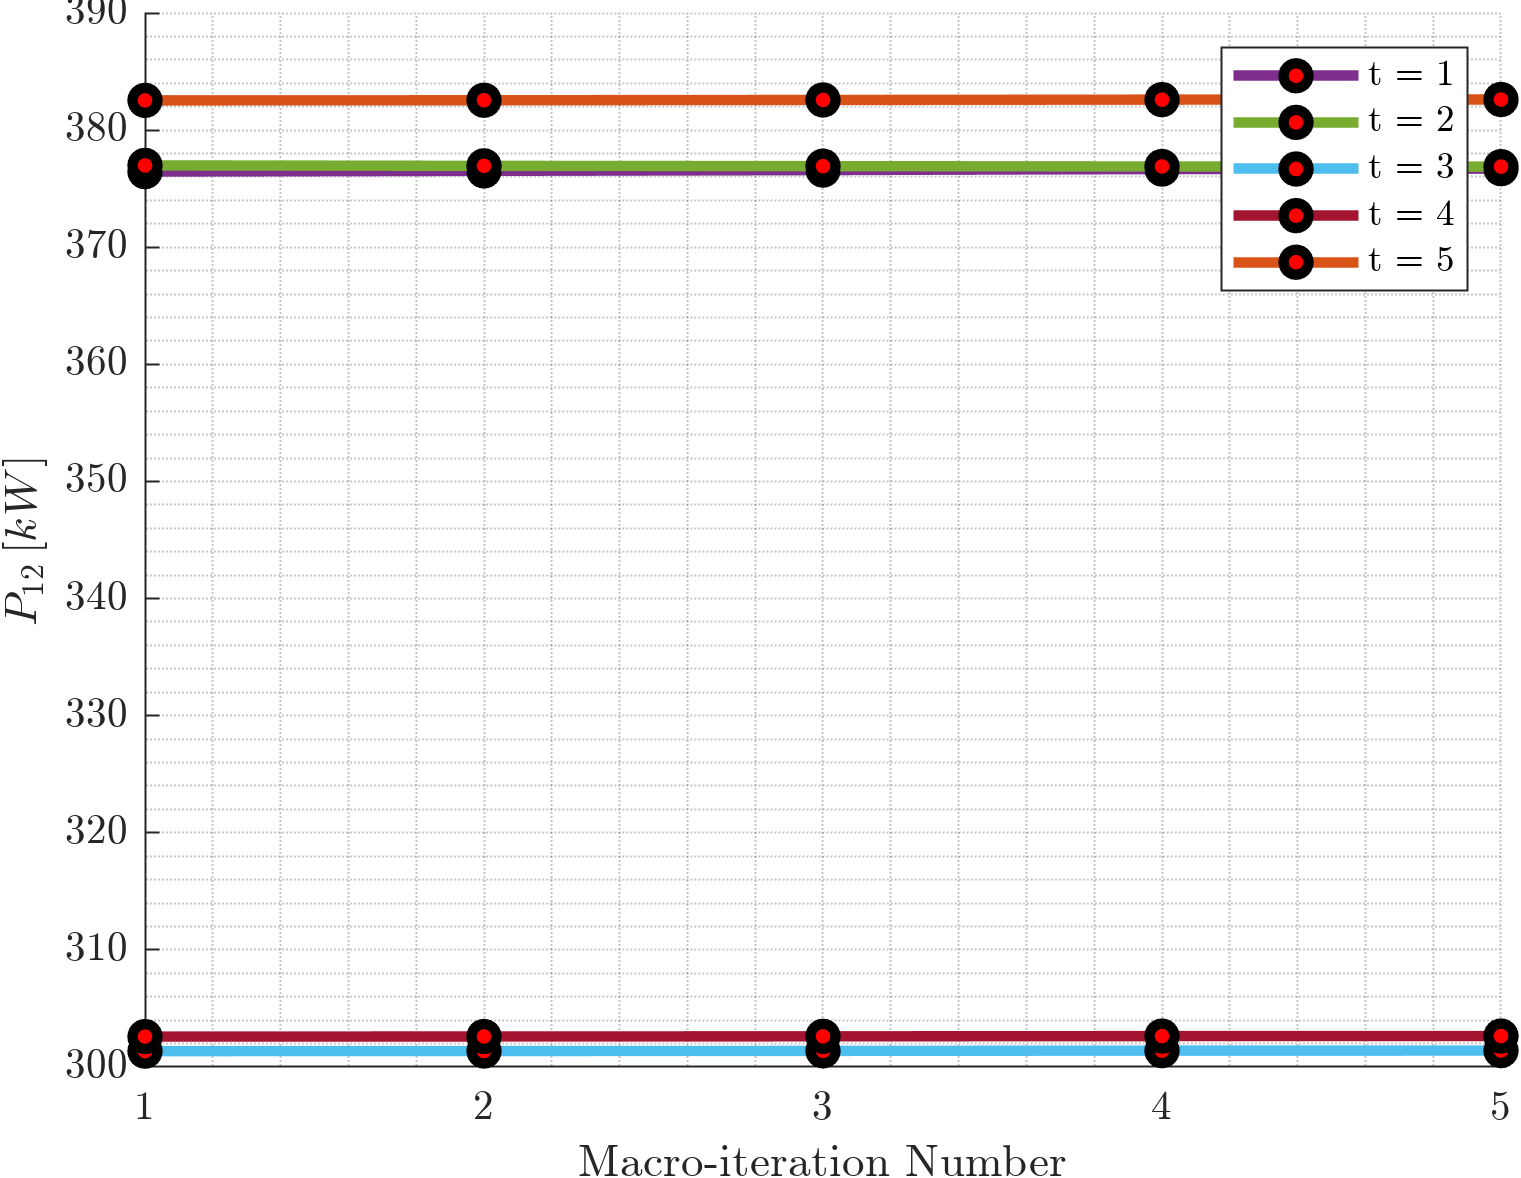
\includegraphics[width=\textwidth,height=0.6\textwidth]{../figures/T5-pv20-batt30-genCost/dopf/convergenceCurves/BoundaryRealPower_vs_t_vs_macroItr_T_5_Areas_2_4_genCost_pv_20_batt_30_crop.png}
%         \caption{\scriptsize Real Power flowing from Area $2$ into Area $4$}
%         \label{fig:real_power_2_4}
%     \end{subfigure}
    
%     % Row 2
%     \begin{subfigure}[b]{0.3\textwidth}
%         \centering
%         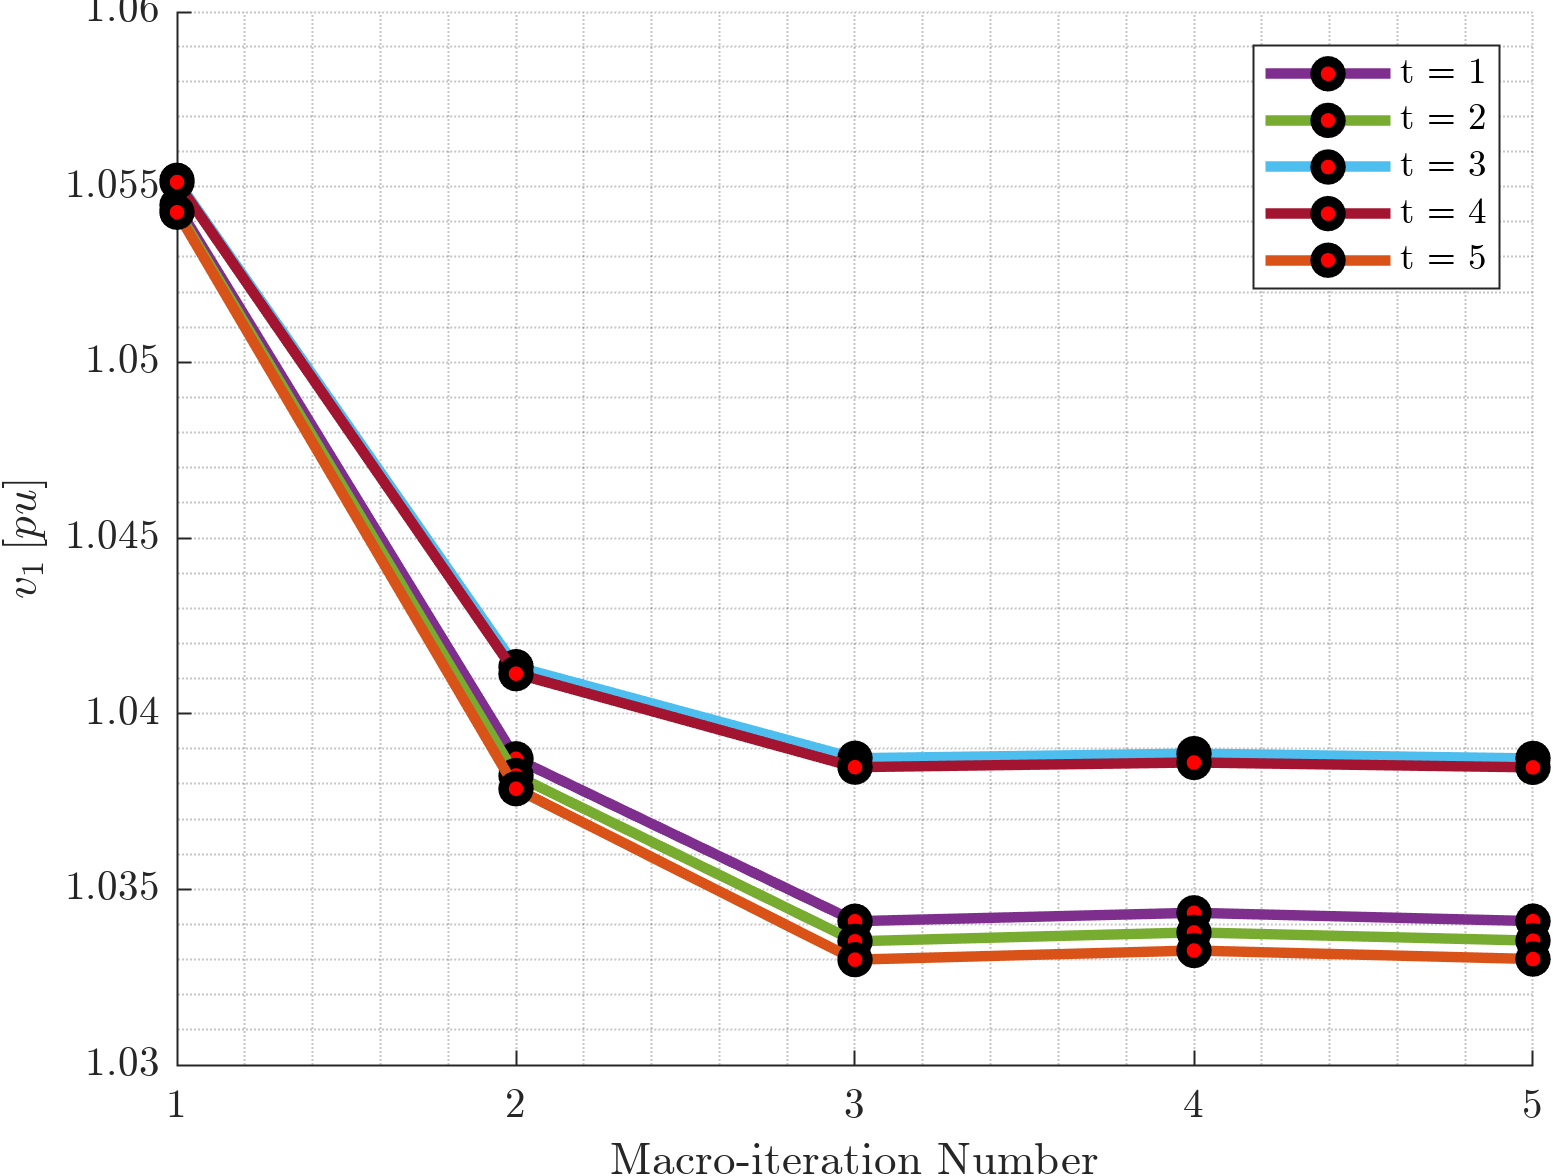
\includegraphics[width=\textwidth,height=0.6\textwidth]{../figures/T5-pv20-batt30-genCost/dopf/convergenceCurves/BoundaryVoltage_vs_t_vs_macroItr_T_5_Areas_1_2_genCost_pv_20_batt_30_crop.png}
%         \caption{\scriptsize Voltage at the PoI of Area $1$ and Area $2$}
%         \label{fig:voltage_1_2}
%     \end{subfigure}
%     \hfill
%     \begin{subfigure}[b]{0.3\textwidth}
%         \centering
%         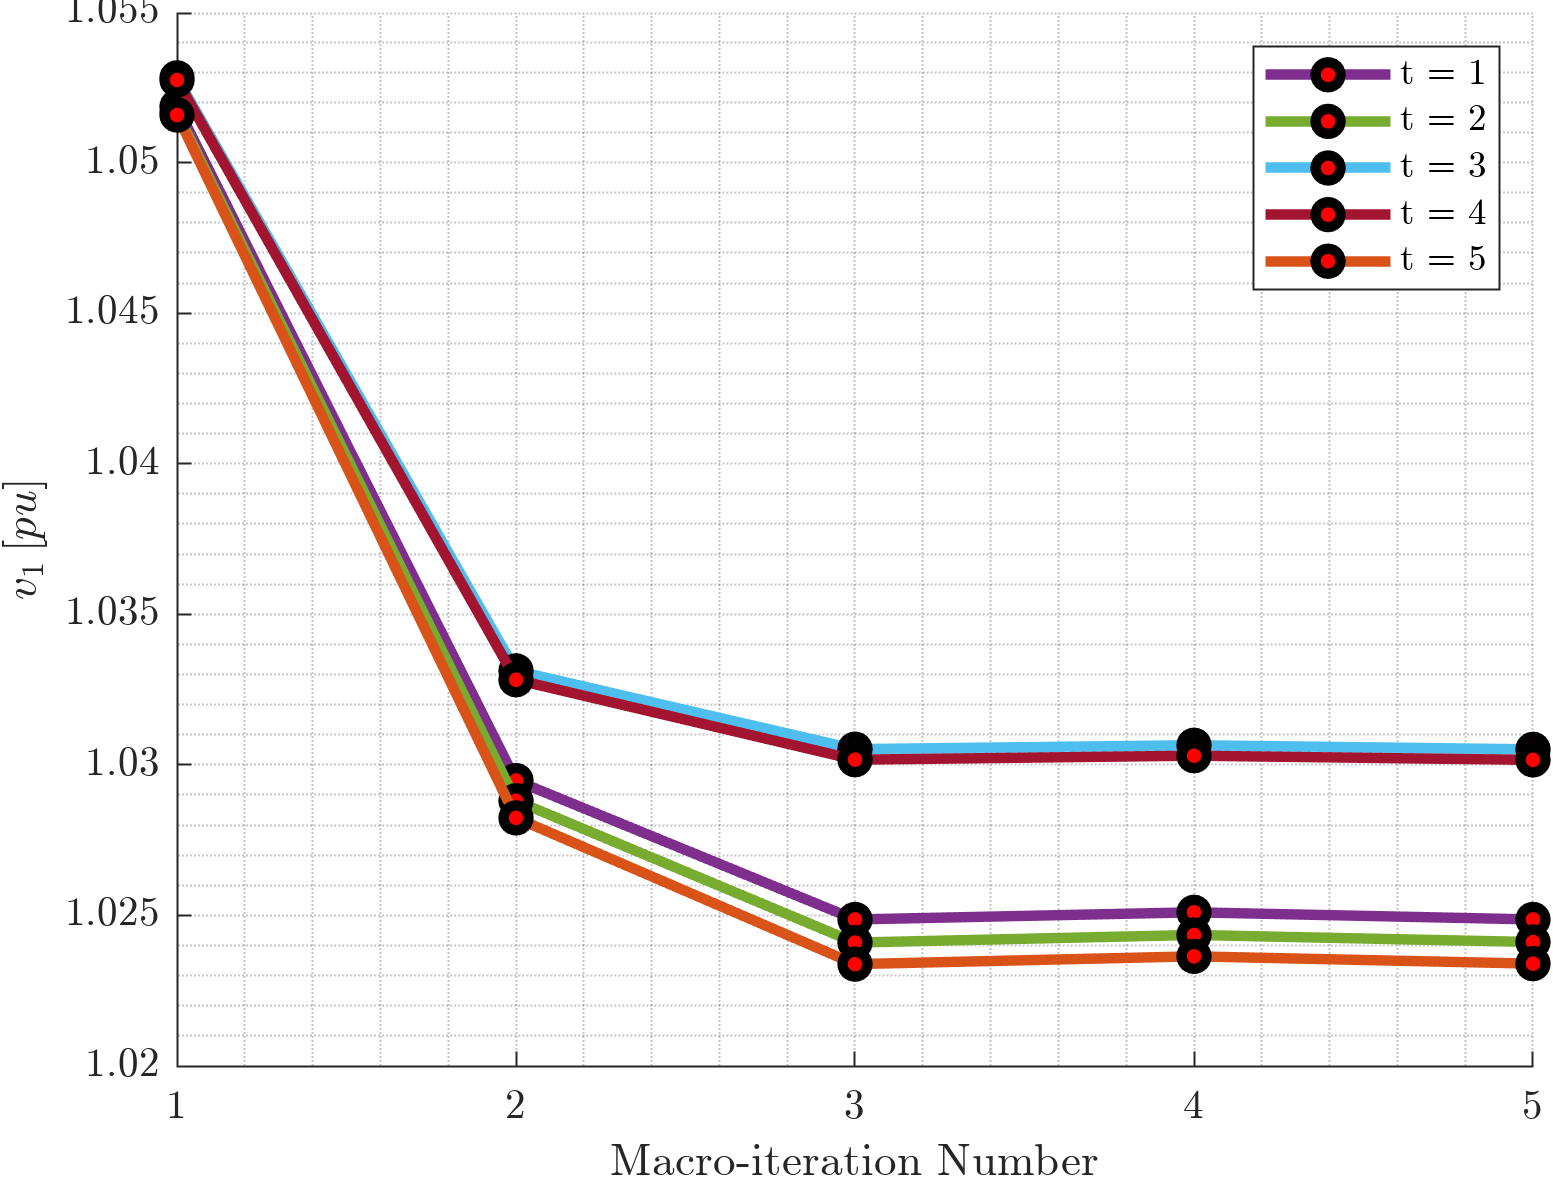
\includegraphics[width=\textwidth,height=0.6\textwidth]{../figures/T5-pv20-batt30-genCost/dopf/convergenceCurves/BoundaryVoltage_vs_t_vs_macroItr_T_5_Areas_1_3_genCost_pv_20_batt_30_crop.png}
%         \caption{\scriptsize Voltage at the PoI of Area $1$ and Area $3$}
%         \label{fig:voltage_1_3}
%     \end{subfigure}
%     \hfill
%     \begin{subfigure}[b]{0.3\textwidth}
%         \centering
%         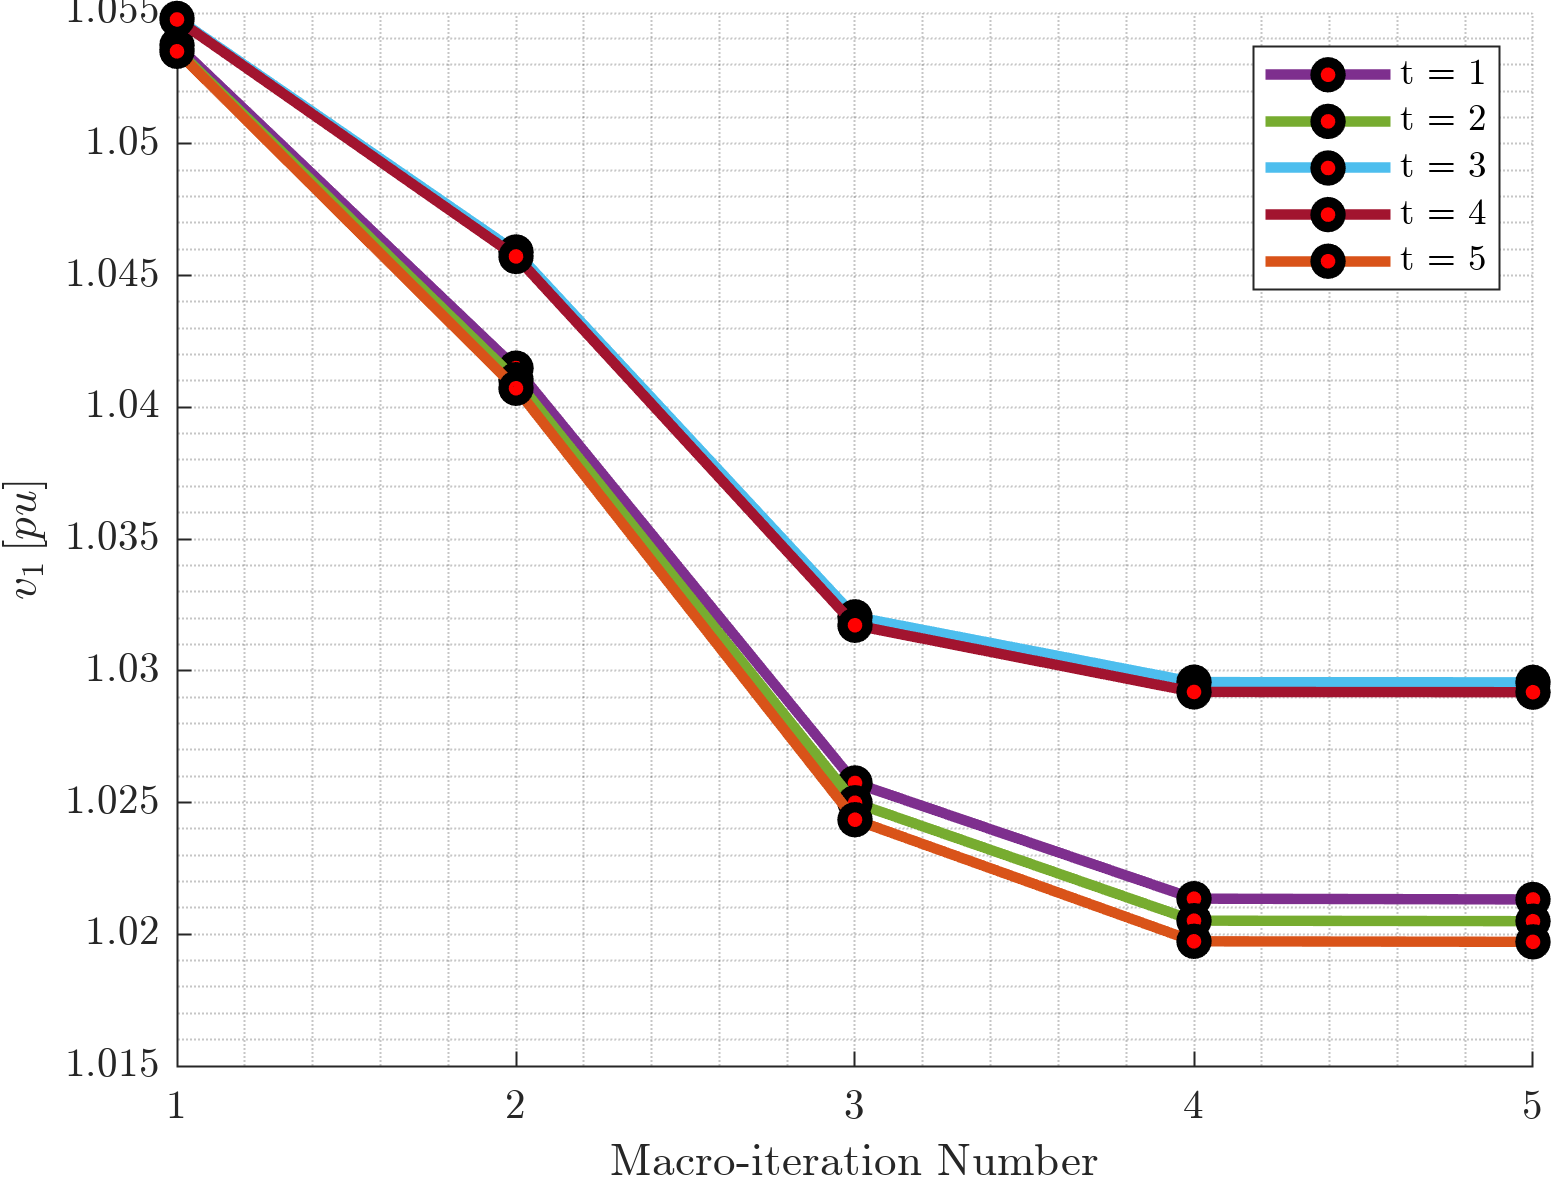
\includegraphics[width=\textwidth,height=0.6\textwidth]{../figures/T5-pv20-batt30-genCost/dopf/convergenceCurves/BoundaryVoltage_vs_t_vs_macroItr_T_5_Areas_2_4_genCost_pv_20_batt_30_crop.png}
%         \caption{\scriptsize Voltage at the PoI of Area $2$ and Area $4$}
%         \label{fig:voltage_2_4}
%     \end{subfigure}

%     \caption{Convergence of Boundary variables with every iteration. Each plot represents a particular variable exchanged between a pair of connected areas. Each line graph within a plot represents a particular time period.}
%     \label{fig:convergenceCurves-5-20-30}
% \end{figure}

% \begin{figure*}[h!] % convergence curves
%     \centering
%     % Row 1
%     \begin{subfigure}[t]{0.32\textwidth}
%         \centering
%         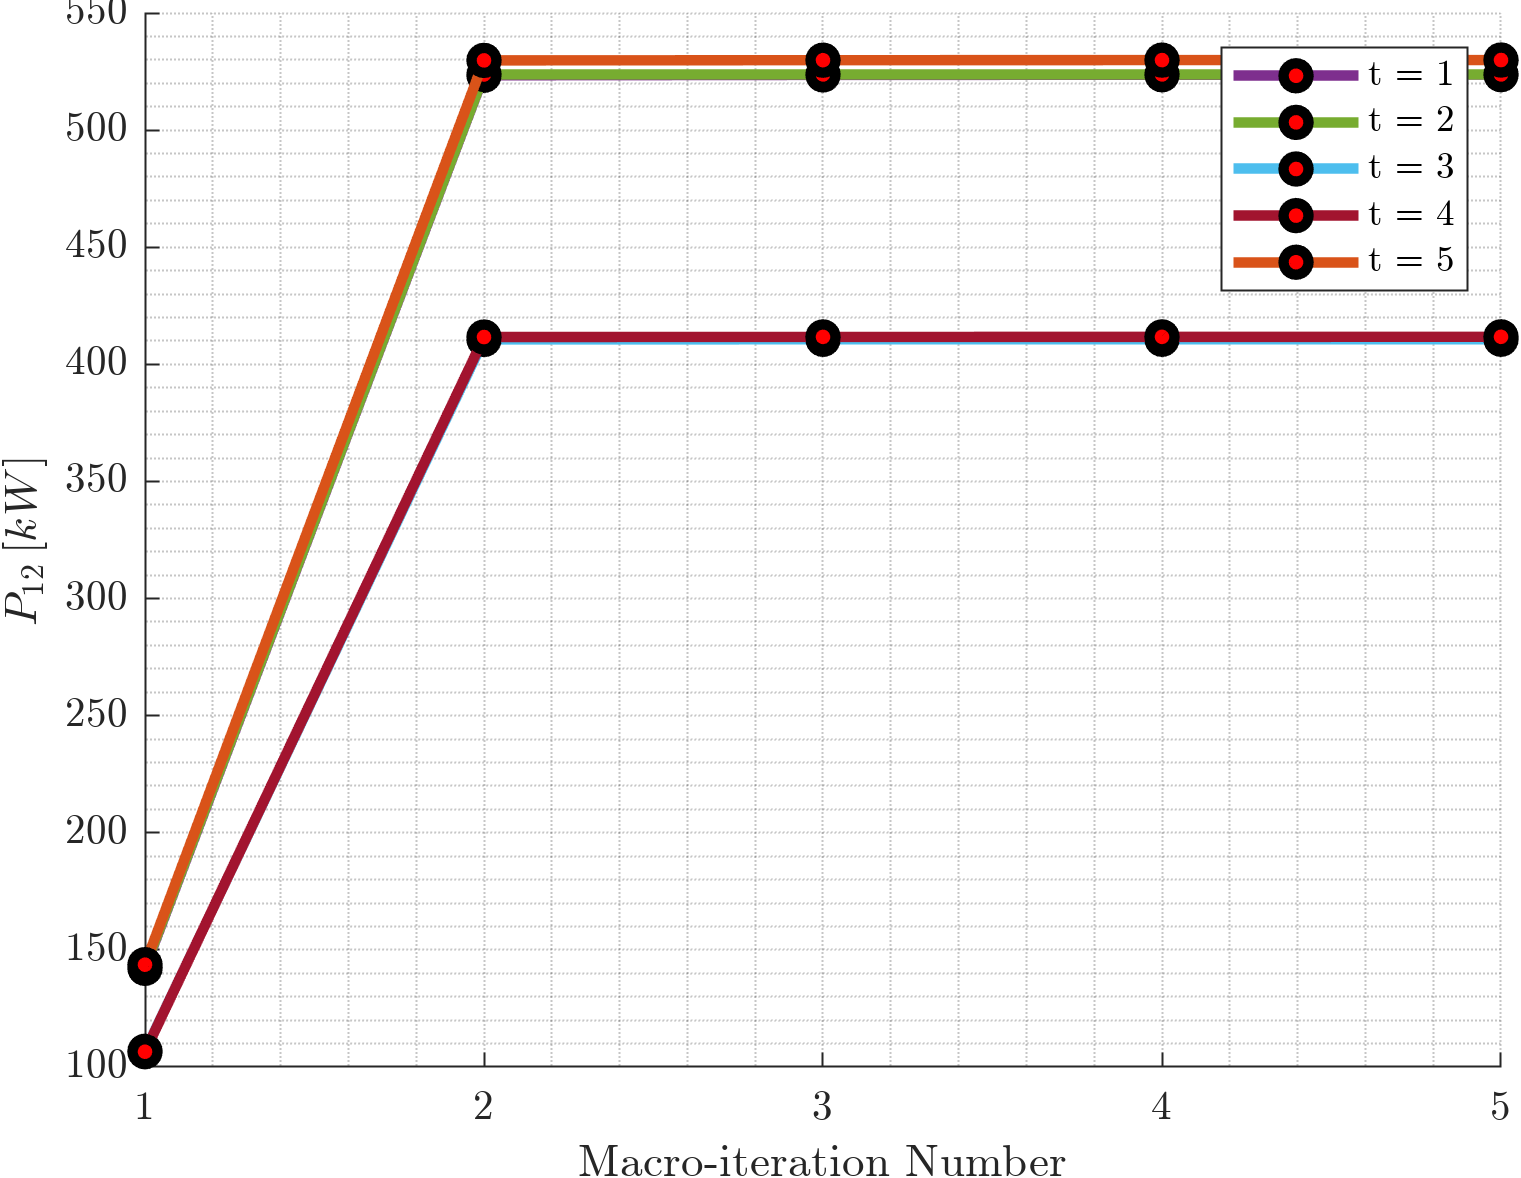
\includegraphics[width=\textwidth]{../figures/T5-pv20-batt30-genCost/dopf/convergenceCurves/BoundaryRealPower_vs_t_vs_macroItr_T_5_Areas_1_2_genCost_pv_20_batt_30_crop.png}
%         \caption{\scriptsize Real Power flowing from Area $1$ into Area $2$}
%         \label{fig:real_power_1_2}
%     \end{subfigure}
%     \hfill
%     \begin{subfigure}[t]{0.32\textwidth}
%         \centering
%         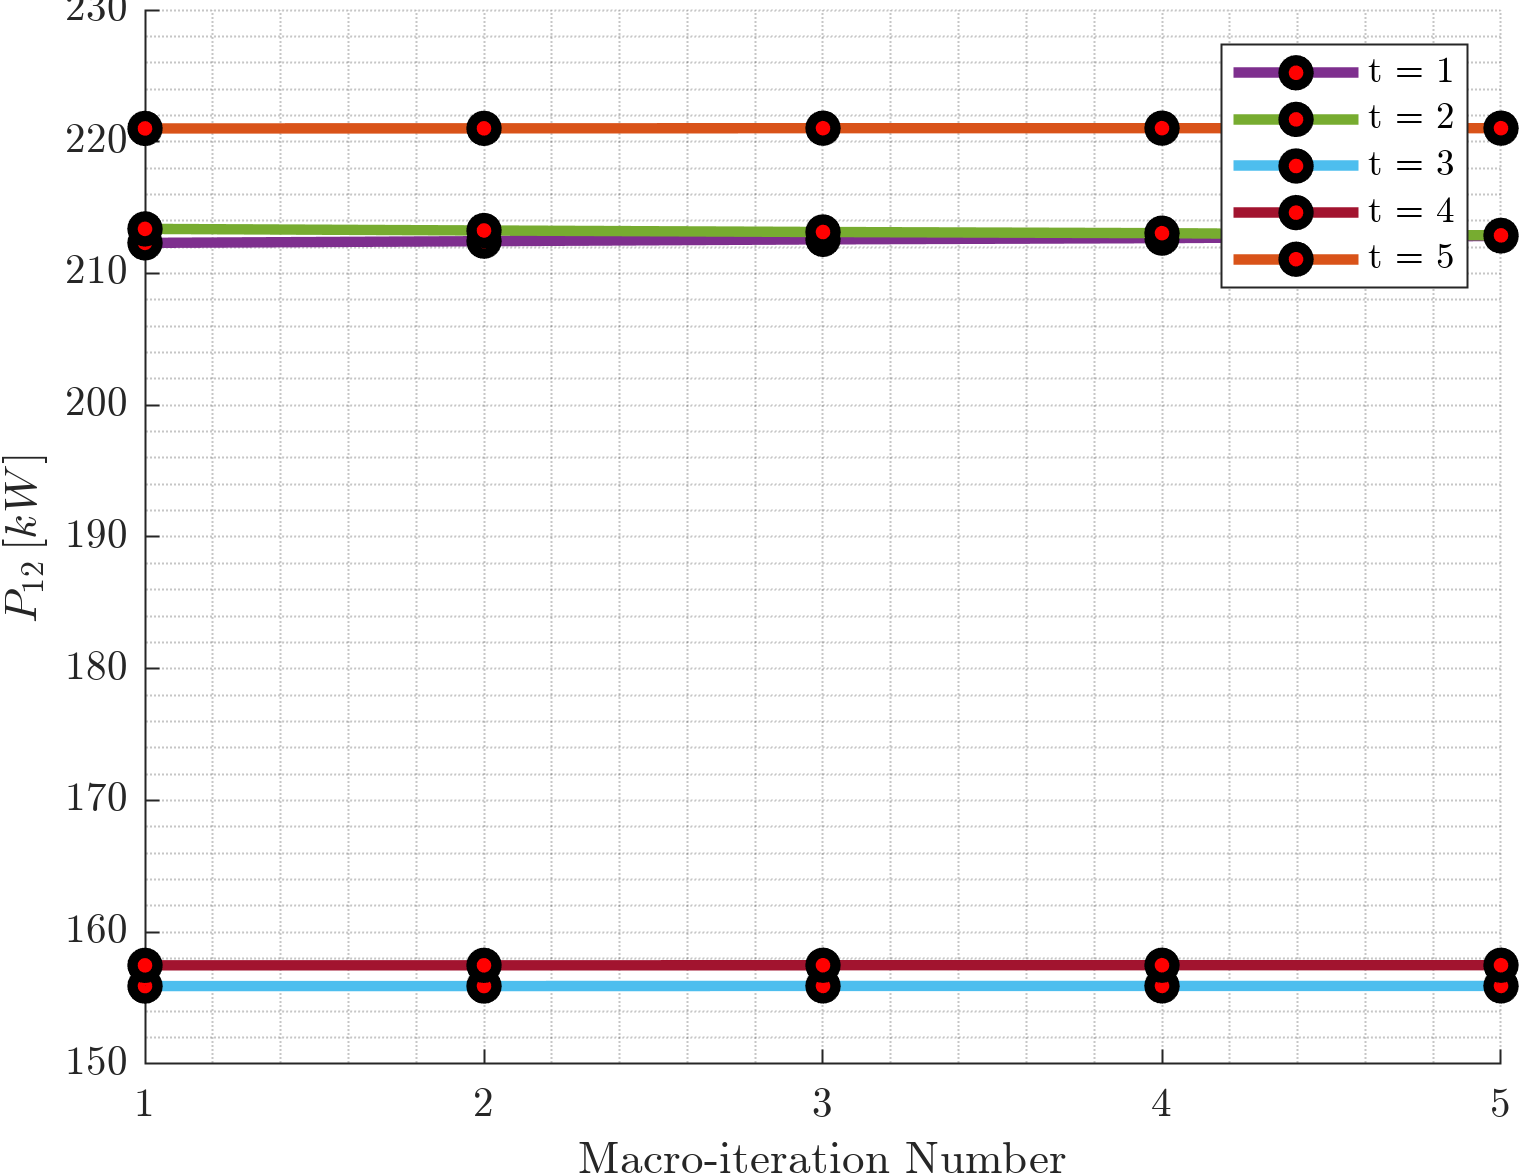
\includegraphics[width=\textwidth]{../figures/T5-pv20-batt30-genCost/dopf/convergenceCurves/BoundaryRealPower_vs_t_vs_macroItr_T_5_Areas_1_3_genCost_pv_20_batt_30_crop.png}
%         \caption{\scriptsize Real Power flowing from Area $1$ into Area $3$}
%         \label{fig:real_power_1_3}
%     \end{subfigure}
%     \hfill
%     \begin{subfigure}[t]{0.32\textwidth}
%         \centering
%         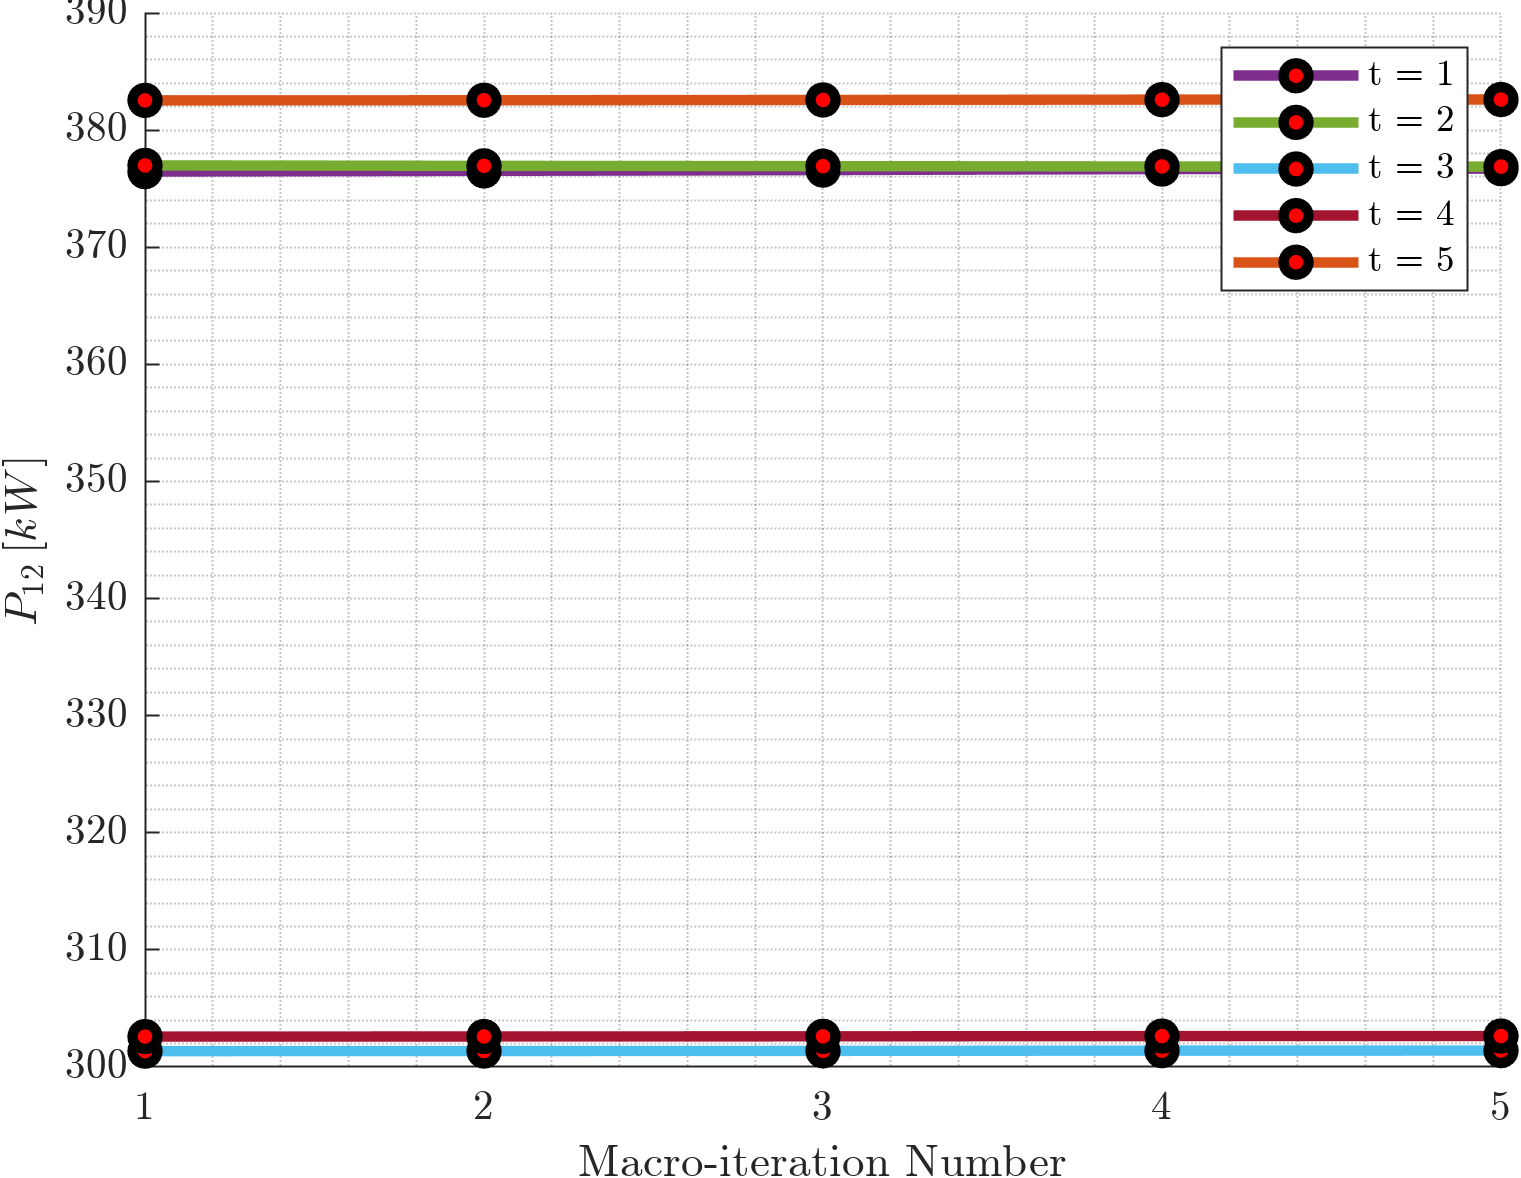
\includegraphics[width=\textwidth]{../figures/T5-pv20-batt30-genCost/dopf/convergenceCurves/BoundaryRealPower_vs_t_vs_macroItr_T_5_Areas_2_4_genCost_pv_20_batt_30_crop.png}
%         \caption{\scriptsize Real Power flowing from Area $2$ into Area $4$}
%         \label{fig:real_power_2_4}
%     \end{subfigure}
    
%     % Row 2
%     \begin{subfigure}[t]{0.32\textwidth}
%         \centering
%         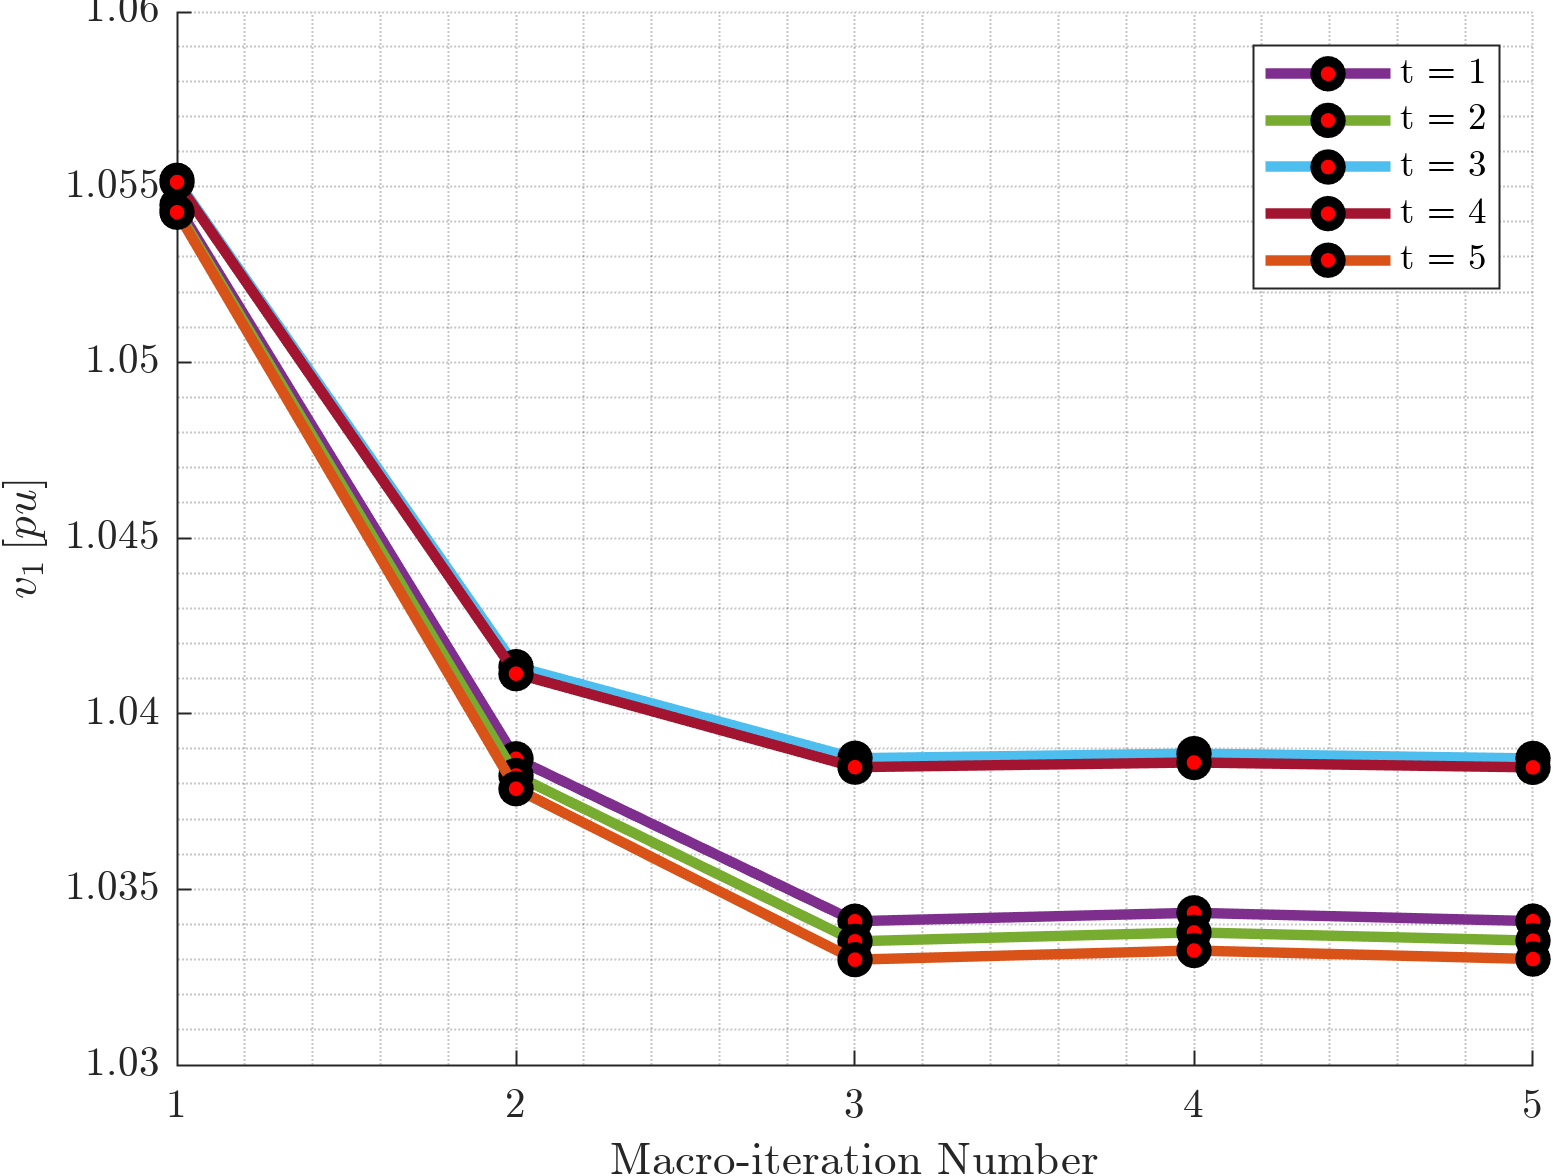
\includegraphics[width=\textwidth]{../figures/T5-pv20-batt30-genCost/dopf/convergenceCurves/BoundaryVoltage_vs_t_vs_macroItr_T_5_Areas_1_2_genCost_pv_20_batt_30_crop.png}
%         \caption{\scriptsize Voltage at the PoI of Area $1$ and Area $2$}
%         \label{fig:voltage_1_2}
%     \end{subfigure}
%     \hfill
%     \begin{subfigure}[t]{0.32\textwidth}
%         \centering
%         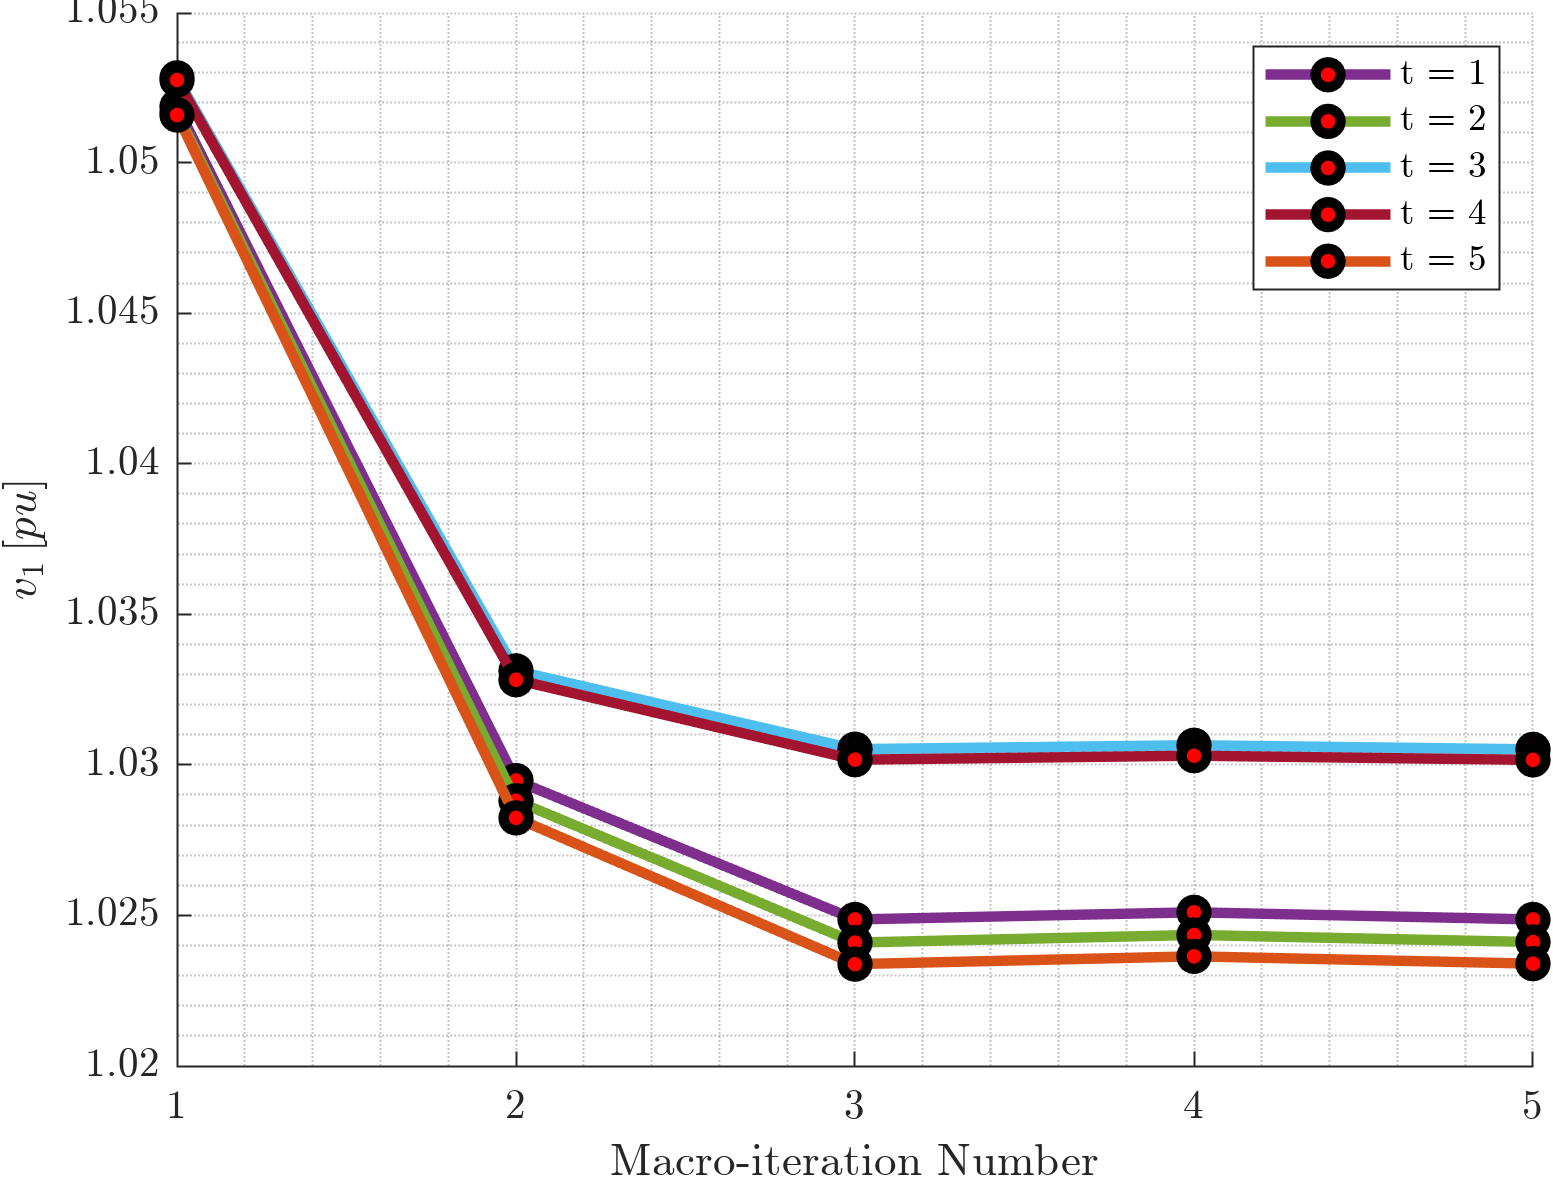
\includegraphics[width=\textwidth]{../figures/T5-pv20-batt30-genCost/dopf/convergenceCurves/BoundaryVoltage_vs_t_vs_macroItr_T_5_Areas_1_3_genCost_pv_20_batt_30_crop.png}
%         \caption{\scriptsize Voltage at the PoI of Area $1$ and Area $3$}
%         \label{fig:voltage_1_3}
%     \end{subfigure}
%     \hfill
%     \begin{subfigure}[t]{0.32\textwidth}
%         \centering
%         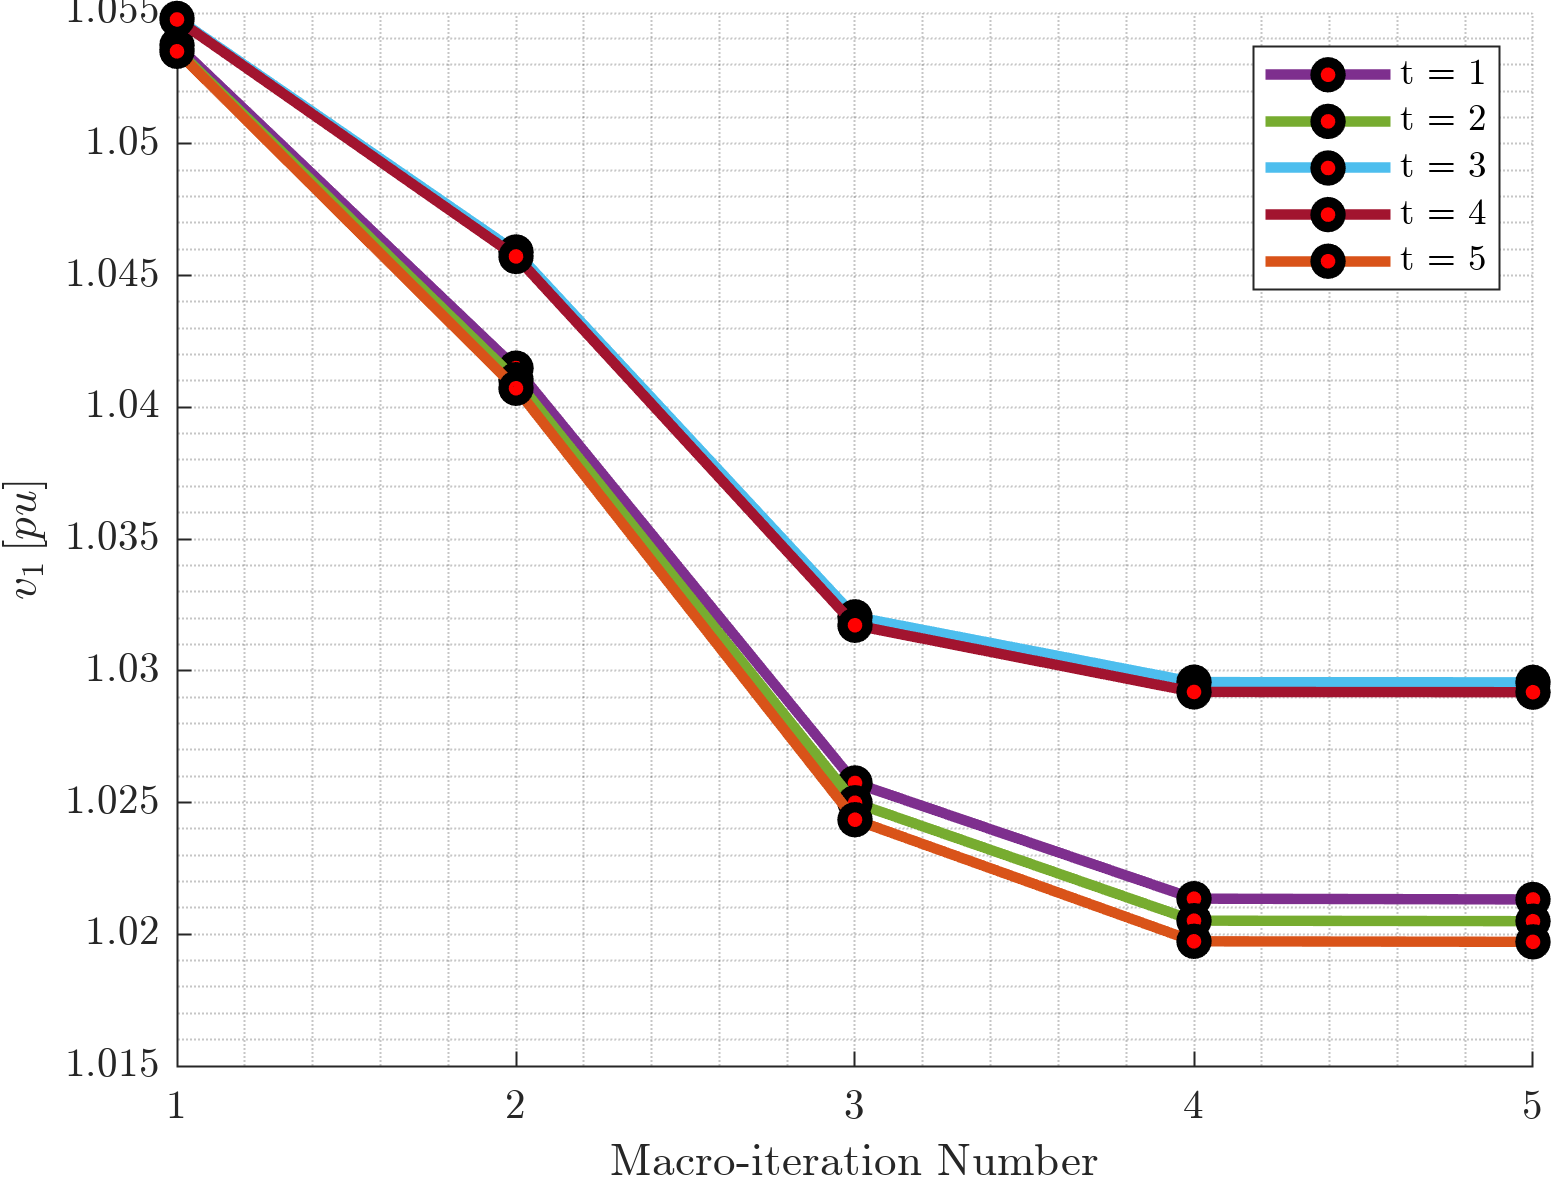
\includegraphics[width=\textwidth]{../figures/T5-pv20-batt30-genCost/dopf/convergenceCurves/BoundaryVoltage_vs_t_vs_macroItr_T_5_Areas_2_4_genCost_pv_20_batt_30_crop.png}
%         \caption{\scriptsize Voltage at the PoI of Area $2$ and Area $4$}
%         \label{fig:voltage_2_4}
%     \end{subfigure}

%     \caption{Convergence of Boundary variables with every iteration. Each plot represents a particular variable exchanged between a pair of connected areas. Each line graph within a plot represents a particular time period.}
%     \label{fig:convergenceCurves-5-20-30}
% \end{figure*}

% \begin{figure}[t]
%     \centering
%     % First plot: Voltage at the PoI of Area 1 and Area 2
%     \begin{subfigure}[b]{\columnwidth}
%         \centering
%         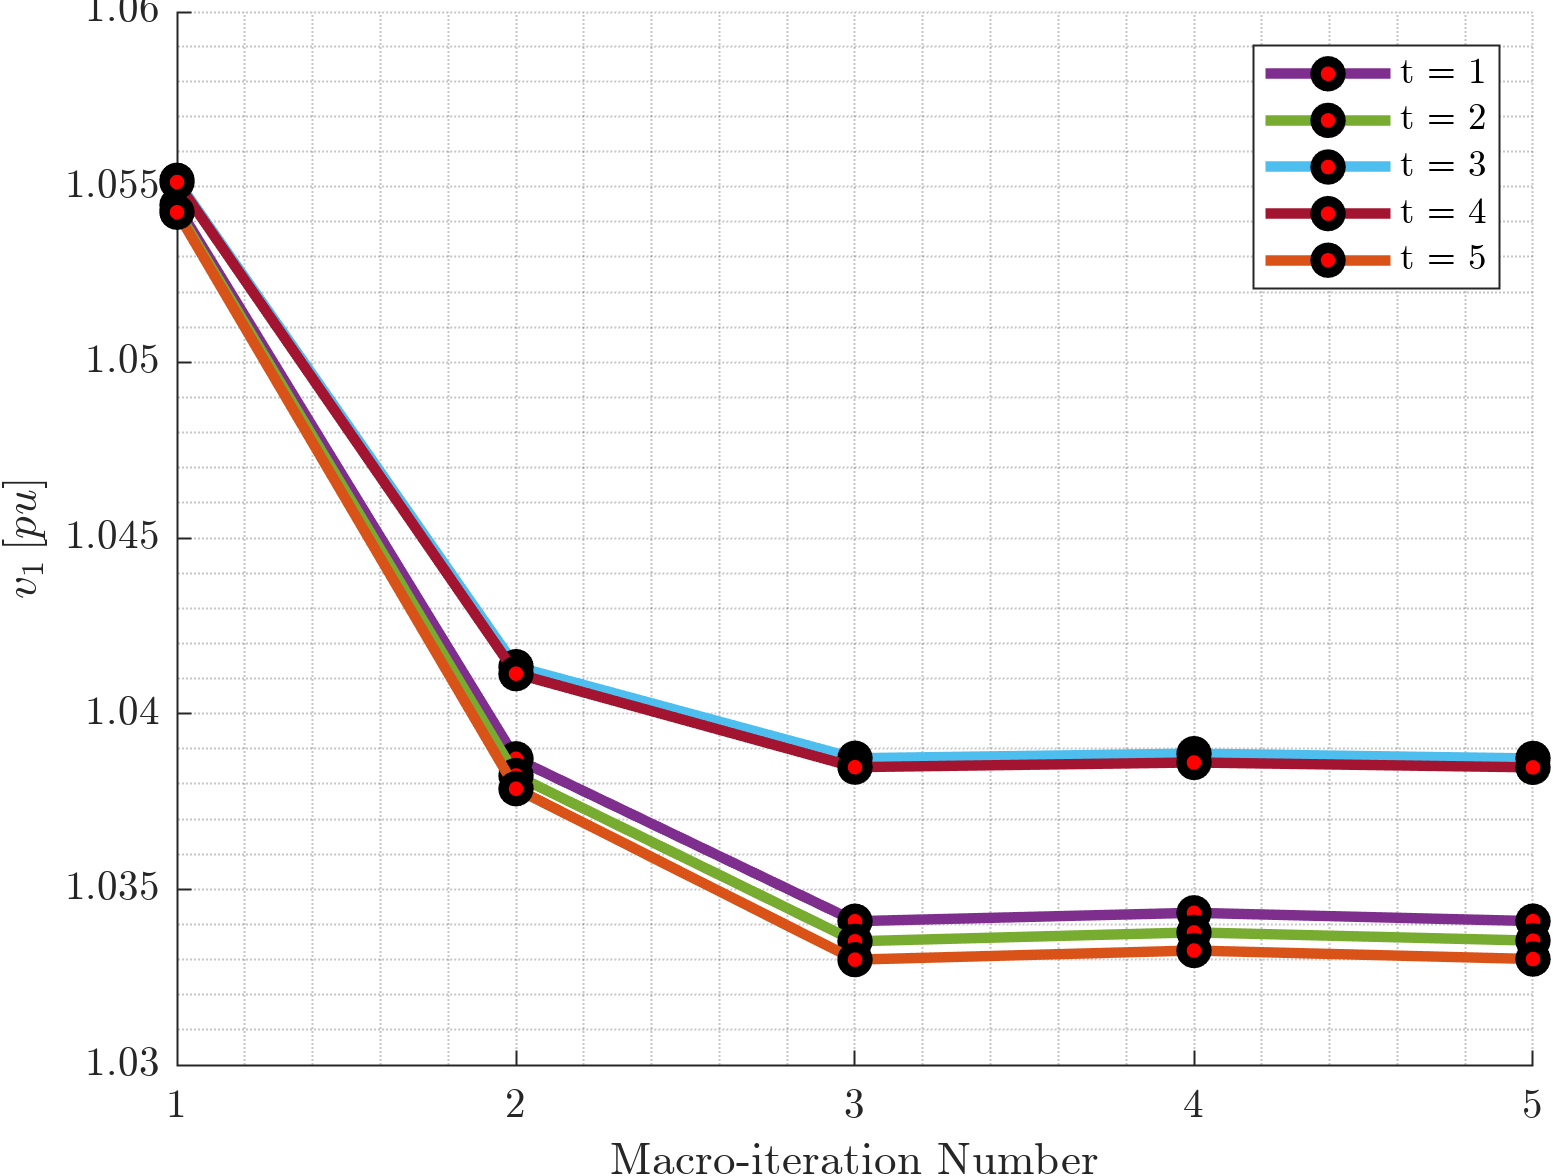
\includegraphics[width=0.8\columnwidth]{../figures/T5-pv20-batt30-genCost/dopf/convergenceCurves/BoundaryVoltage_vs_t_vs_macroItr_T_5_Areas_1_2_genCost_pv_20_batt_30_crop.png}
%         \caption{\scriptsize Shared voltage data from Area $1$ to Area $2$}
%         \label{fig:voltage_1_2}
%     \end{subfigure}
%     \vfill
%     % Second plot: Real Power flowing from Area 2 into Area 4
%     \begin{subfigure}[b]{\columnwidth}
%         \centering
%         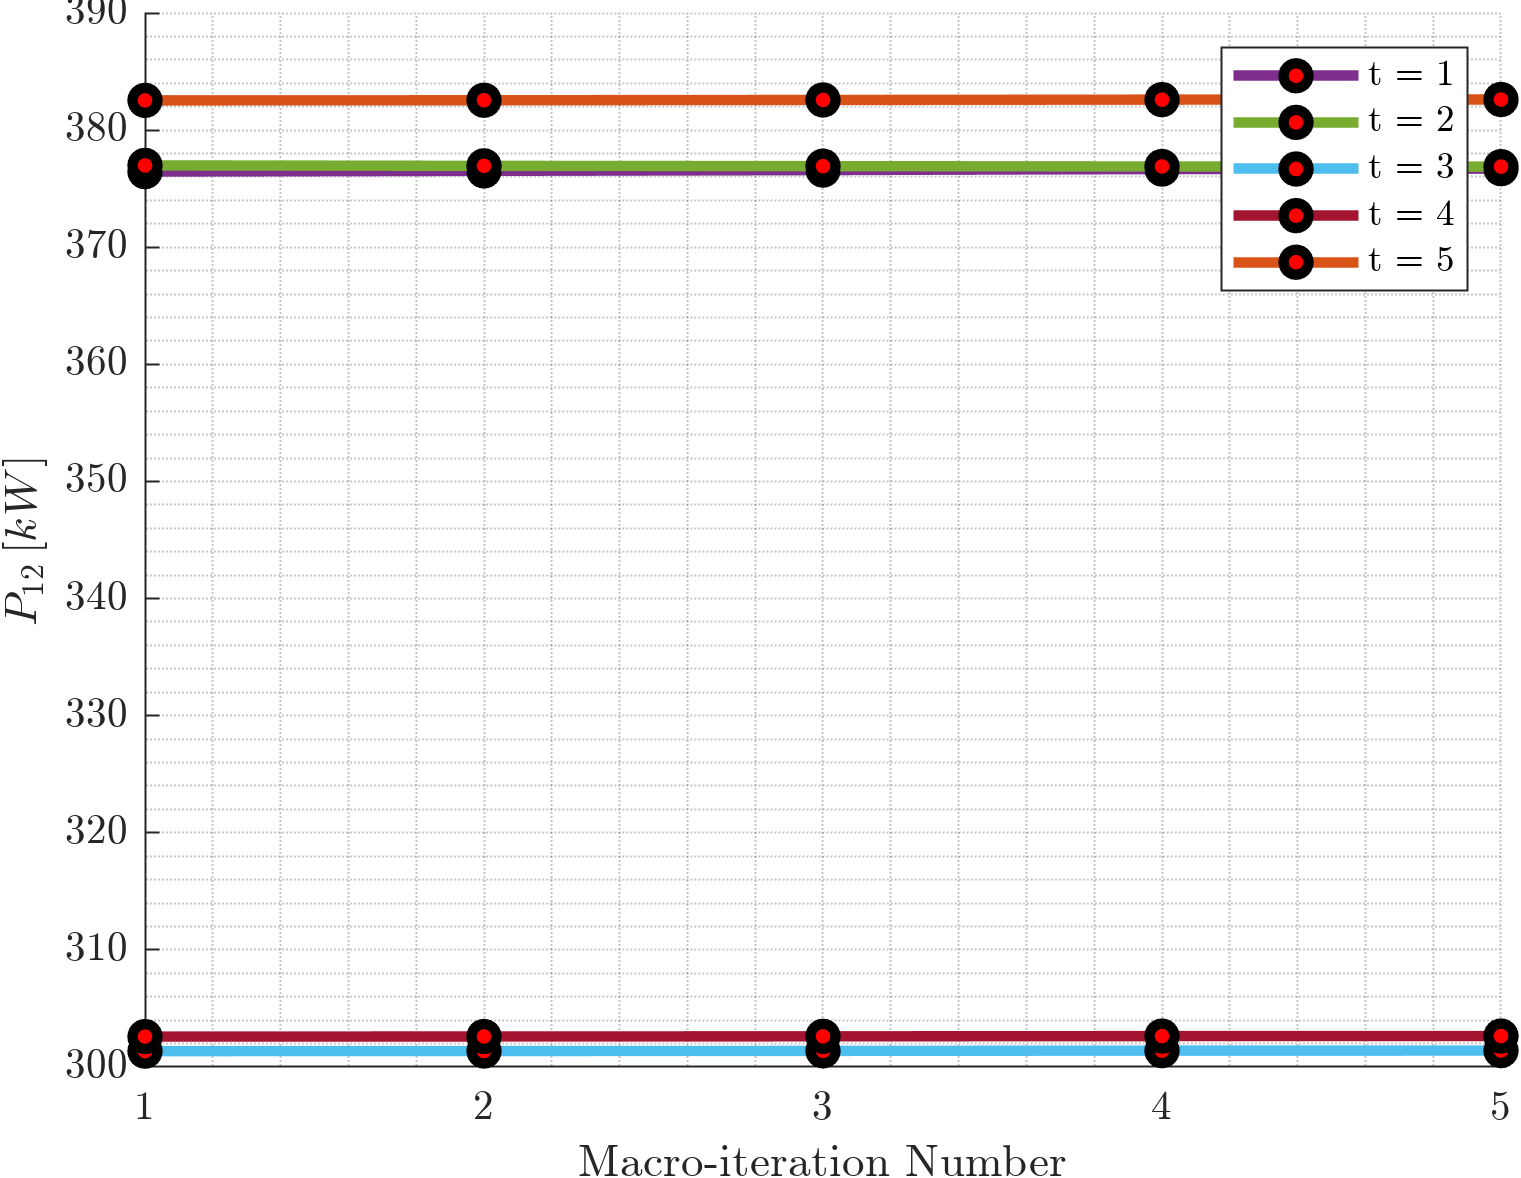
\includegraphics[width=0.8\columnwidth]{../figures/T5-pv20-batt30-genCost/dopf/convergenceCurves/BoundaryRealPower_vs_t_vs_macroItr_T_5_Areas_2_4_genCost_pv_20_batt_30_crop.png}
%         \caption{\scriptsize Shared real power data from Area $4$ into Area $2$}
%         \label{fig:real_power_2_4}
%     \end{subfigure}
    
%     \caption{Convergence of boundary variables. Each plot represents a particular variable exchanged between a pair of connected areas. Each line graph within a plot represents a particular time period.}
%     \label{fig:convergenceCurves-5-20-30}
%     \vspace{-4mm}
% \end{figure}

% \begin{figure}[t]
%     \centering
%     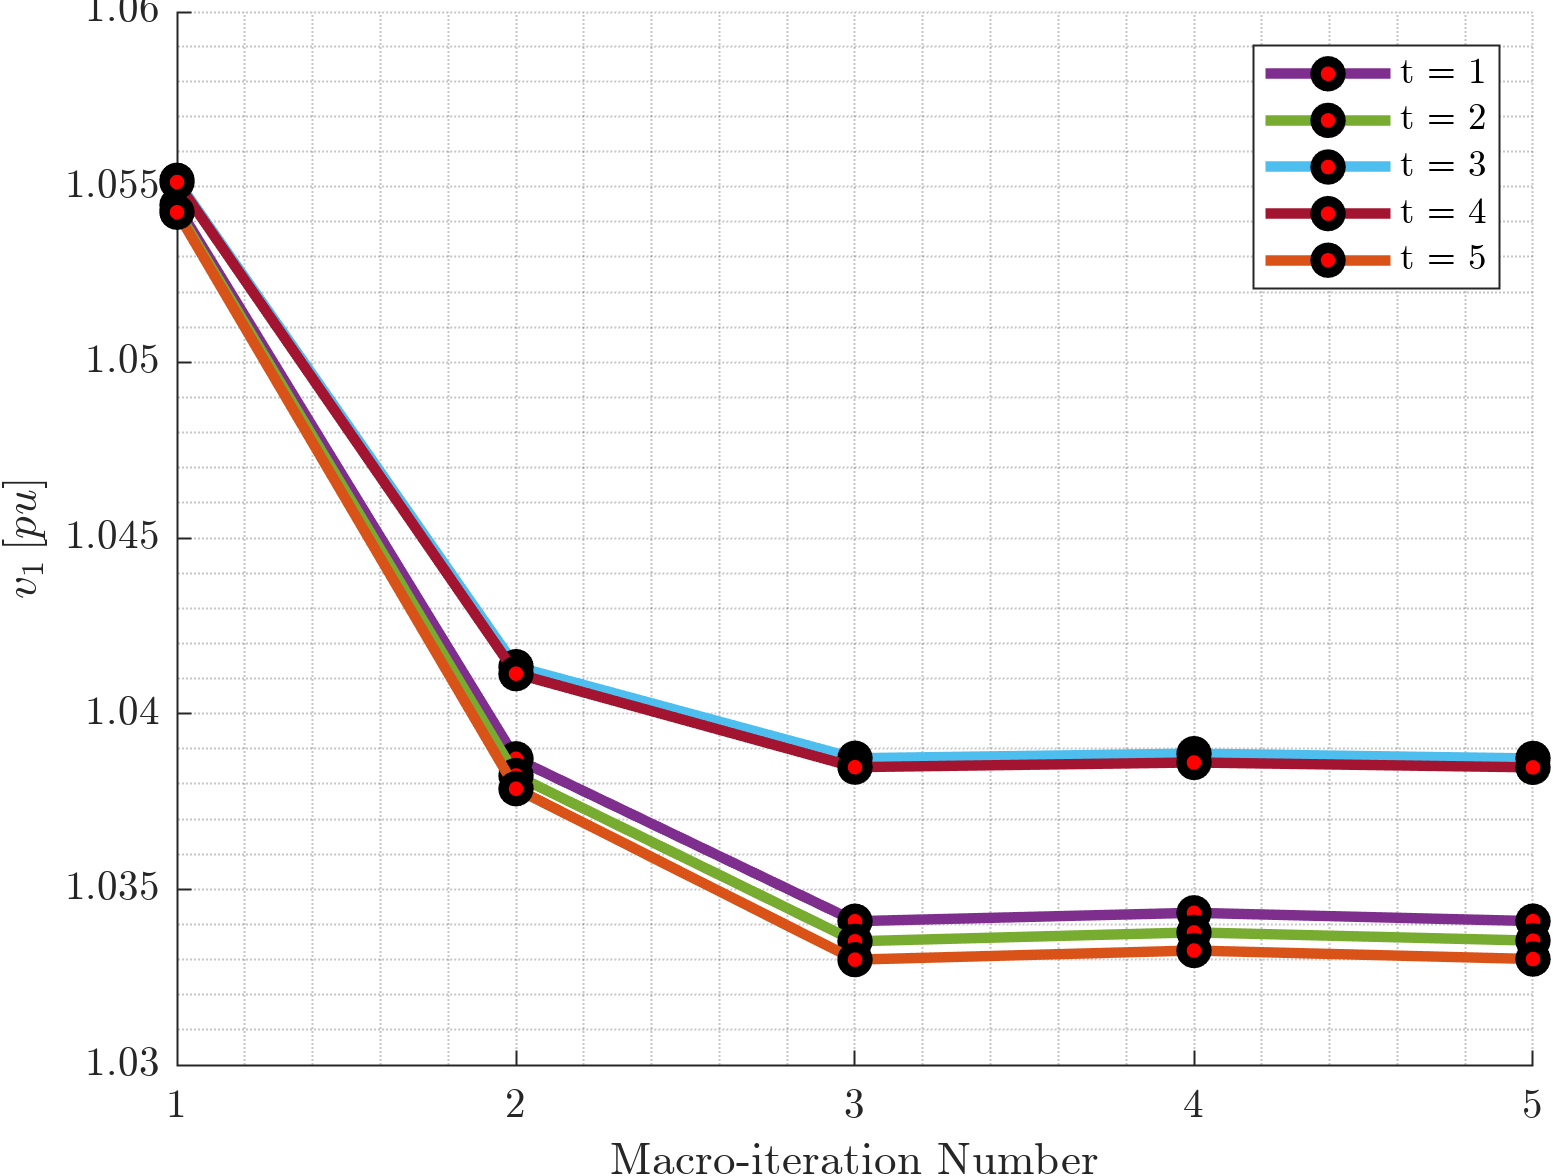
\includegraphics[width=0.8\columnwidth]{../figures/T5-pv20-batt30-genCost/dopf/convergenceCurves/BoundaryVoltage_vs_t_vs_macroItr_T_5_Areas_1_2_genCost_pv_20_batt_30_crop.png}
%     \caption{ Shared voltage data from Area $1$ to Area $2$.}
%     \label{fig:voltage_1_2}
%     \vspace{-4mm}
% \end{figure}

% \begin{figure}[t]
%     \centering
%     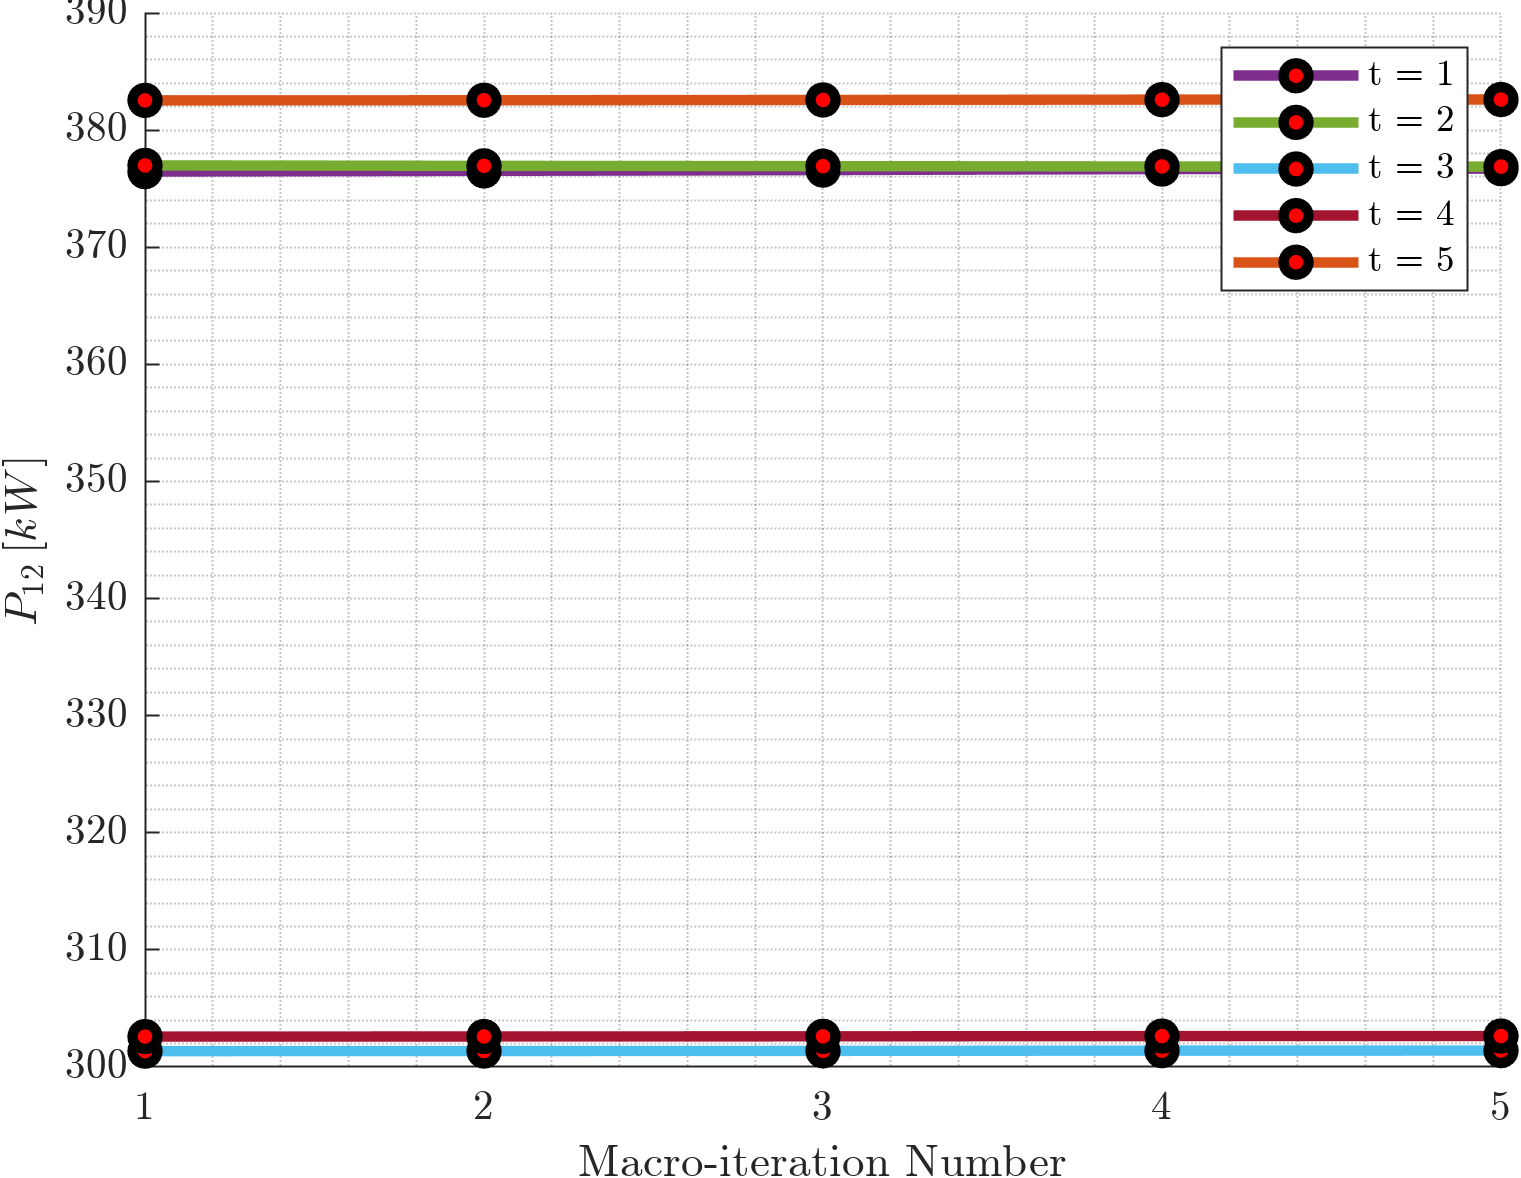
\includegraphics[width=0.8\columnwidth]{../figures/T5-pv20-batt30-genCost/dopf/convergenceCurves/BoundaryRealPower_vs_t_vs_macroItr_T_5_Areas_2_4_genCost_pv_20_batt_30_crop.png}
%     \caption{Shared real power data from Area $4$ into Area $2$.}
%     % \label{fig:real_power_2_4}
%   \label{fig:convergenceCurves-5-20-30}
%     \vspace{-4mm}
% \end{figure}

% \begin{figure}[t] % output variable convergence curve
%     \centering
%     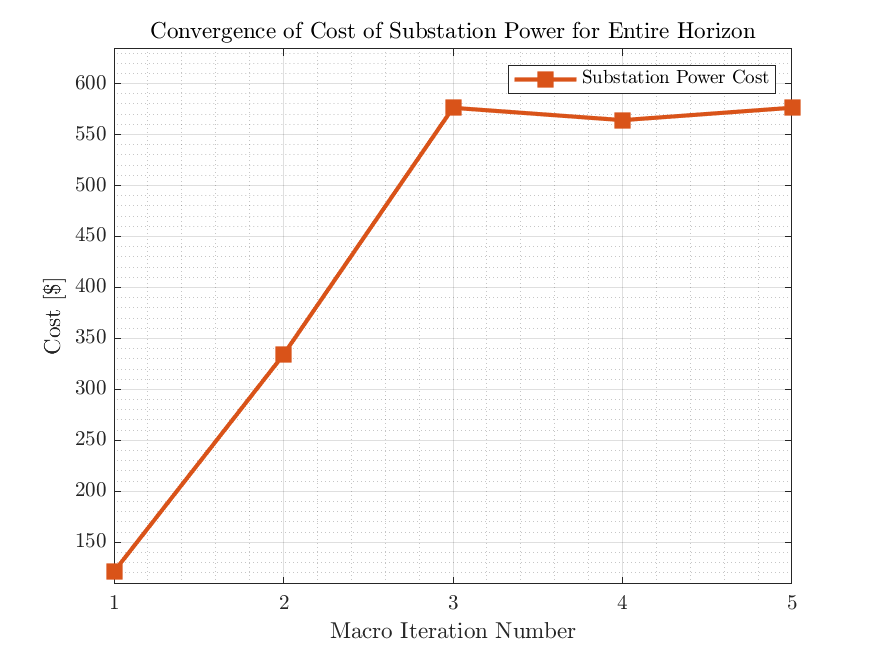
\includegraphics[height=0.25\textheight]{../figures/T5-pv20-batt30-genCost/dopf/outputCurves/ObjectiveConvergenceCurves_Horizon_5.png}
%     \caption{Convergence of objective function value with each MPDOPF iteration}
%     \label{fig:outputConvergence-5-pv20-batt30-genCost}
%     \vspace{-4mm}
% \end{figure}

% \subsection{Scalability Analysis} \label{subsec:scalabilityAnalysis}

% To demonstrate the scalability of the proposed algorithm, additional simulations were conducted over a 10-hour time horizon. \Cref{fig:inputCurve-10} shows the forecasted profiles for load, solar irradiance and cost of substation power over the 10-hour horizon. The simulation results are summarized in \Cref{table:opt-10-20-30} and \Cref{table:feas-copf-10-20-30}.

% From the comparison against MPCOPF in \Cref{table:opt-10-20-30}, it can again be seen that MPDOPF is able to converge to the same optimal solution as MPCOPF. The computational speed up is even more pronounced than for the $5$ time-period simulation. 
% % It is noted that the solution time increased drastically for MPCOPF with the increasing length of the study horizon. However, the solution time increment for MPDOPF is comparatively less. Therefore, the proposed spatially distributed MPOPF framework is scalable to some extent.
% It was observed that the solution time for MPCOPF increased significantly with the length of the study horizon, whereas the increase in solution time for MPDOPF was comparatively smaller. This indicates that the proposed spatially distributed MPOPF framework is scalable to a certain extent.

% \begin{figure}[t]
%     \centering
%     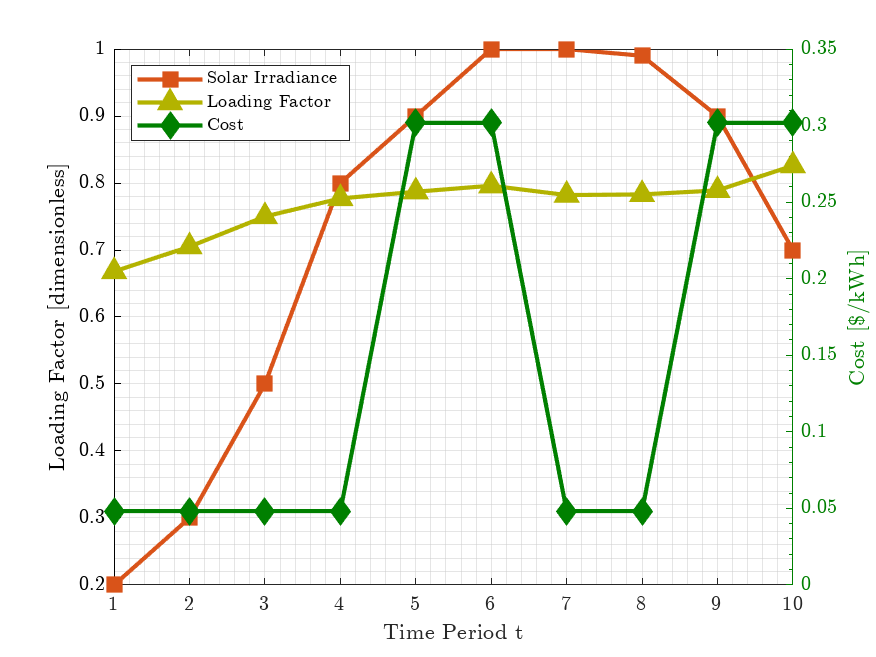
\includegraphics[height=0.25\textheight]{../figures/T10-inputCurves/InputCurves_Horizon_10.png}
%     \caption{Forecasts for demand power, irradiance and cost of substation power over a 10 hour Horizon}
%     \label{fig:inputCurve-10}
%     % \vspace{-4mm}
% \end{figure}


\begin{table}[H]
    \centering
    \caption{Comparison between Nonlinear BFM and LinDistFlow - $10$ hour}
    \begin{tabular}{|l|c|c|}
    \hline
    \textbf{Metric} & \textbf{Nonlinear BFM} & \textbf{LinDistFlow} \\ \hline
    Largest subproblem & \multicolumn{2}{c|}{} \\ \hline
    \quad Decision variables & {6300} & {2640} \\ \hline
    \quad Linear constraints & {11636} & {4891} \\ \hline
    \quad Nonlinear constraints & {1270} & {530} \\ \hline
    Simulation results  & \multicolumn{2}{c|}{} \\ \hline
    \quad Substation power cost (\$) & 1197.87 & 1197.87 \\ \hline
    \quad Substation real power (kW) & 8544.28 & 8544.04 \\ \hline
    \quad Line loss (kW) & 148.67 & 148.94 \\ \hline
    \quad Substation reactive power (kVAR) & 1092.39 & 1252.03 \\ \hline
    \quad PV reactive power (kVAR) & 222.59 & 139.81 \\ \hline
    \quad Battery reactive power (kVAR) & 388.52 & 310.94 \\ \hline
    Computation  & \multicolumn{2}{c|}{} \\ \hline
    \quad Number of Iterations & - & 5 \\ \hline
    \quad Total Simulation Time (s) & 4620.73 & 358.69 \\ \hline
    \end{tabular}
    \label{table:opt-10-20-30}
    % \vspace{-1mm}
\end{table}

% Again, as can be seen in \Cref{table:feas-copf-10-20-30} comparison against OpenDSS has yielded small discrepancies, attesting to the feasibility of the solution. 

\begin{table}[t]
    \centering
    \caption{ACOPF feasibility analyses - $24$ hour}
    \begin{tabular}{|l|c|c|}
    \hline
    \textbf{Metric} & \textbf{BFM-NL} & \textbf{LinDistFlow} \\ \hline
    Max. all-time discrepancy & \multicolumn{2}{c|}{} \\ \hline
    \quad Voltage (pu) & 0000 & 0.002056 \\ \hline
    \quad Line loss (kW) & 0000 & 1.807435 \\ \hline
    \quad Substation power (kW) & 0000 & 32.362217 \\ \hline
    \quad Substation reactive power (kVAR) & 0000 & 64.402519 \\ \hline
    \end{tabular}
    \label{table:feas-copf-10-20-30}
    \vspace{-3mm}
\end{table}


% \begin{figure}[h!]
%     \centering
%     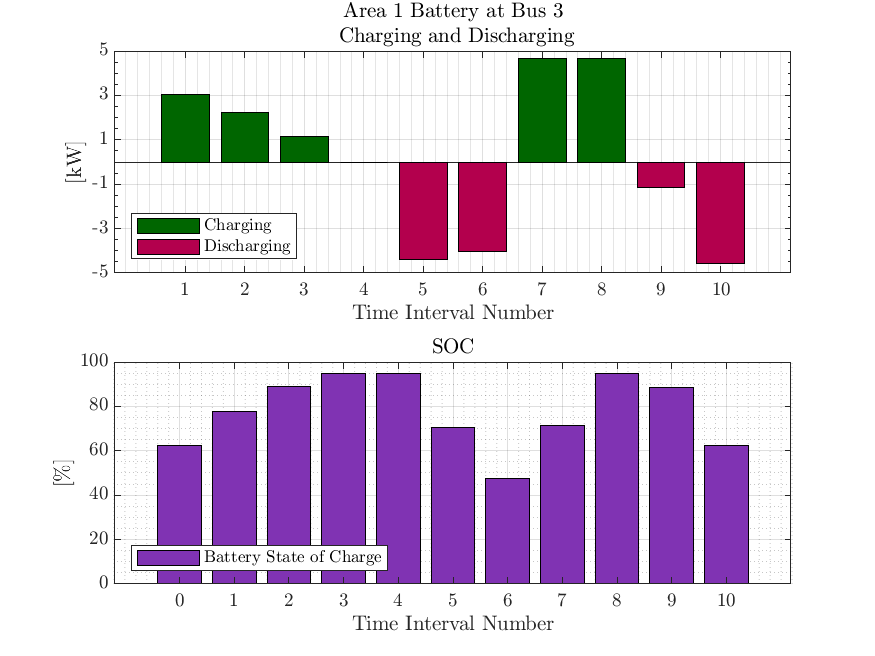
\includegraphics[width=\linewidth]{../figures/T10-pv20-batt30-genCost/dopf/BatteryPlots/macroItr_5_genCost_Battery_1_alpha_0.001.png}
%     \caption{Charging-Discharging and SOC graphs for Battery at Bus 3 located in Area 1 obtained via MPDOPF}
%     \label{fig:batt-plot-dopf-10-20-30-genCost}
% \end{figure}


\end{document}
